\documentclass[a4paper, 11pt]{article}
\usepackage{graphicx}
\usepackage[utf8]{vietnam}
\usepackage{indentfirst}
\usepackage{longtable}
\usepackage{fdsymbol}
\usepackage{color}
\usepackage{biblatex}
\usepackage{fullpage}
\usepackage{blindtext}
\usepackage{hyperref}
\usepackage{multicol}
\usepackage{caption}
\usepackage{amsmath}
\usepackage[table]{xcolor}
\usepackage{geometry}
\usepackage{listings}

\definecolor{codegreen}{rgb}{0,0.6,0}
\definecolor{codegray}{rgb}{0.5,0.5,0.5}
\definecolor{codepurple}{rgb}{0.58,0,0.82}
\definecolor{mintedbackground}{rgb}{0.95,0.95,0.95}

\lstdefinestyle{mystyle}{
    backgroundcolor=\color{mintedbackground},
    commentstyle=\color{codegreen},
    keywordstyle=\color{magenta},
    numberstyle=\tiny\color{codegray},
    stringstyle=\color{codepurple},
    basicstyle=\ttfamily\footnotesize,
    breakatwhitespace=false,
    breaklines=true,
    captionpos=b,
    keepspaces=true,
    numbers=left,
    numbersep=5pt,
    showspaces=false,
    showstringspaces=false,
    showtabs=false,
    tabsize=4,
    texcl=false,
}

\lstset{style=mystyle}

\setcounter{MaxMatrixCols}{20}

\title{Bài tập tổng hợp cuối kỳ môn quản trị hệ thống}
\author{Kim Minh Thắng B2007210}

\begin{document}
\maketitle
\tableofcontents
\listoffigures
\listoftables
\lstlistoflistings

\newpage

\section*{Mô tả bài tập}

Công ty Straw Hat chuyên kinh doanh hải sản có nhu cầu xây dựng hệ thống mạng cục bộ phục vụ cho công việc của công ty như sau:

\begin{minipage}{\linewidth}
    \captionsetup{type=figure}
    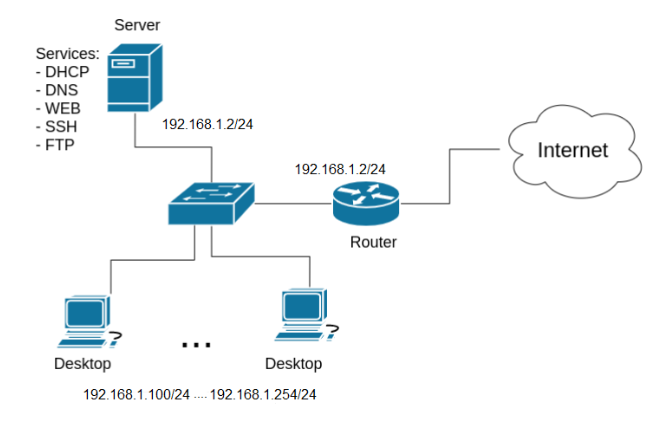
\includegraphics[width=\linewidth]{images/networks.png}
    \caption{Sơ đồ hệ thống mạng của công ty Straw Hat}
\end{minipage}

\section{Cài đặt và cấu hình Server/Desktop}

\subsection{(10\%) Sử dụng phần mềm VirtualBox cài đặt Server và Desktop:}

\begin{itemize}
    \item[--] Tạo 1 NAT Network tên "QTHT" có địa chỉ mạng là 192.168.1.0/24. Tắt dịch vụ DHCP có sẵn trên NAT Network "QTHT".
    \item[--] Tạo 2 máy ảo với thông tin như sau: \hfill \\
          \begin{minipage}{\linewidth}
              \begin{multicols}{2}
                  \begin{minipage}{\linewidth}
                      \captionsetup{type=table}
                      \caption{Cấu hình máy Server}
                      \centering
                      \begin{tabular}{| p{.4\linewidth} | p{.4\linewidth} |}
                          \hline
                          \textbf{Hostname}         & Server                                                               \\
                          \hline

                          \textbf{Hệ điều hành}     & CentOS 9                                                             \\
                          \hline

                          \textbf{CPU / RAM / DISK} & 1core/2G/10G \newline Hoặc tùy chỉnh theo cấu hình máy của sinh viên \\
                          \hline

                          \textbf{Network}          & NAT Network \newline Name: "QTHT"                                    \\
                          \hline

                          \textbf{IP}               & 192.168.1.2                                                          \\
                          \hline

                          \textbf{Subnet mask}      & 255.255.255.0                                                        \\
                          \hline

                          \textbf{Gateway}          & 192.168.1.1                                                          \\
                          \hline

                          \textbf{DNS}              & 192.168.1.1                                                          \\
                          \hline
                      \end{tabular}
                  \end{minipage}

                  \begin{minipage}{\linewidth}
                      \captionsetup{type=table}
                      \caption{Cấu hình máy Desktop}
                      \centering
                      \begin{tabular}{| p{.4\linewidth} | p{.5\linewidth} |}
                          \hline
                          \textbf{Hostname}                                              & Desktop                                                              \\
                          \hline

                          \textbf{Hệ điều hành}                                          & Lubuntu 22.04, \newline hoặc bất kỳ hệ điều hành khác                \\
                          \hline

                          \textbf{CPU / RAM / DISK}                                      & 1core/2G/10G \newline Hoặc tùy chỉnh theo cấu hình máy của sinh viên \\
                          \hline

                          \textbf{Network}                                               & NAT Network \newline Name: "QTHT"                                    \\
                          \hline

                          \textbf{IP \newline Subnet mask \newline Gateway \newline DNS} & Cấu hình tự động sử dụng dịch vụ DHCP                                \\
                          \hline
                      \end{tabular}
                  \end{minipage}
              \end{multicols}
          \end{minipage}

    \item[--] Trong quá trình cài hệ điều hành CentOS 9, tạo 1 tài khoản với username là <Mã số sinh viên>; firstname và lastname là họ tên của sinh viên. Cấp quyền quản trị (sudo) cho tài khoản. Sử dụng tài khoản vừa tạo để thực hiện bài tập tổng hợp (không dùng tài khoản root).
    \item[--] Tắt dịch vụ tường lửa trên Server.
\end{itemize}

\subsubsection{Tạo 1 NAT Network tên "QTHT"}

\begin{minipage}{\linewidth}
    \captionsetup{type=figure}
    \centering
    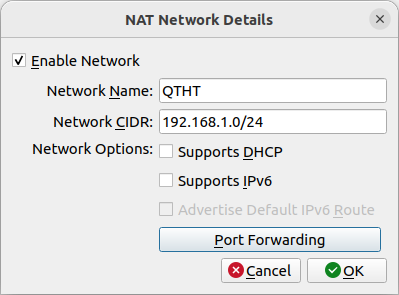
\includegraphics[width=8cm]{images/create-nat.png}
    \caption{Cấu hình NAT Network QTHT}
\end{minipage}

Để tắt dịch vụ DHCP mặc định của NAT Network trong VirtualBox, ta bỏ tích tùy chọn "Supports DHCP".

\subsubsection{Tạo 2 máy ảo Server và Desktop}

\begin{enumerate}
    \item \textbf{Server có cấu hình như sau:}
          \begin{itemize}
              \item Hệ điều hành: CentOS 9
              \item CPU: 1 Core \textit{(Hình \ref{figure:server-processor})}
              \item Ram: 4GB \textit{(Hình \ref{figure:server-ram})}
              \item Disk: 20GB \textit{(Hình \ref{figure:server-disk})}
              \item Network: NAT Network "QTHT" \textit{(Hình \ref{figure:server-network-1})}
              \item IPv4: 192.168.1.2 \textit{(Hình \ref{figure:server-network-2})}
              \item Subnet mask: 255.255.255.0 \textit{(Hình \ref{figure:server-network-2})}
              \item Gateway: 192.168.1.1 \textit{(Hình \ref{figure:server-network-2})}
              \item DNS: 192.168.1.1 \textit{(Hình \ref{figure:server-network-2})}
          \end{itemize}

          \begin{minipage}
              {\linewidth}
              \captionsetup{type=figure}
              \centering
              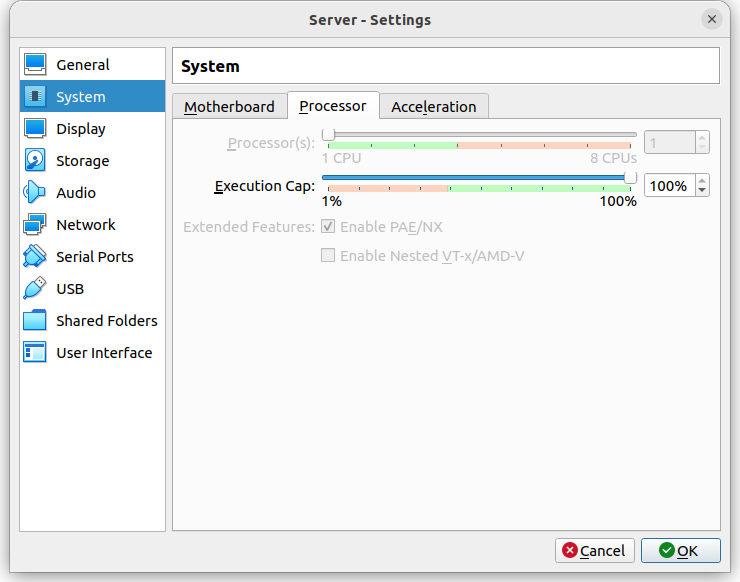
\includegraphics[width=\linewidth]{images/server-processor.png}
              \caption{Số Core CPU cho Server}
              \label{figure:server-processor}
          \end{minipage}

          \begin{minipage}{\linewidth}
              \captionsetup{type=figure}
              \centering
              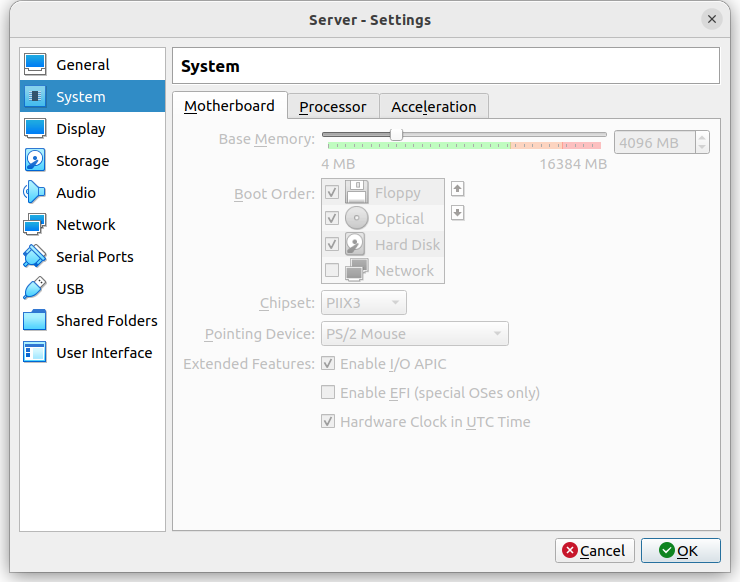
\includegraphics[width=\linewidth]{images/server-ram.png}
              \caption{Dung lượng RAM cho Server}
              \label{figure:server-ram}
          \end{minipage}

          \begin{minipage}
              {\linewidth}
              \captionsetup{type=figure}
              \centering
              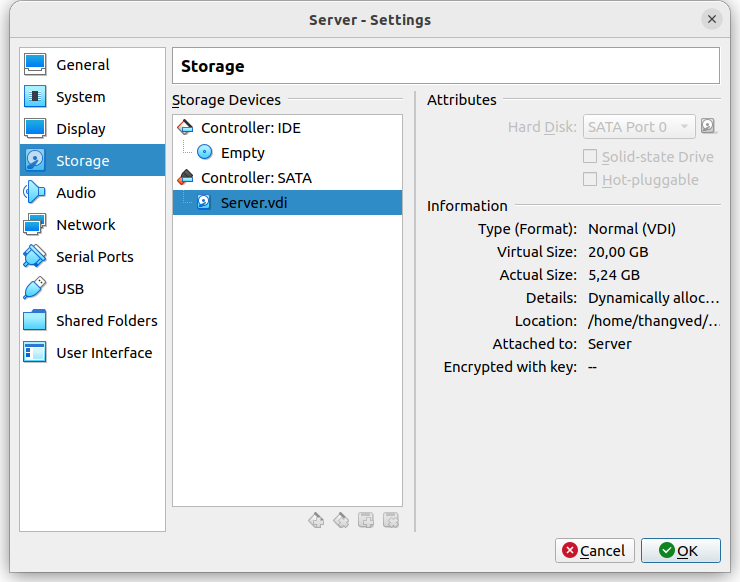
\includegraphics[width=\linewidth]{images/server-disk.png}
              \caption{Dung lượng ổ cứng cho Server}
              \label{figure:server-disk}
          \end{minipage}

          \begin{minipage}
              {\linewidth}
              \captionsetup{type=figure}
              \centering
              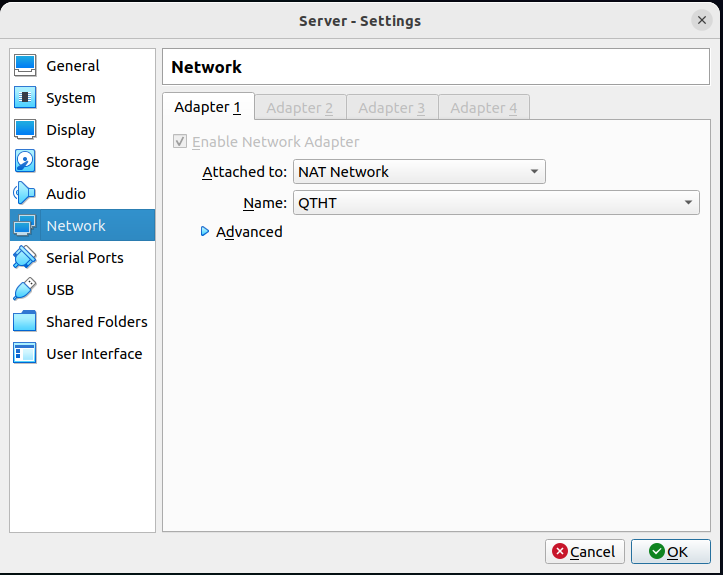
\includegraphics[width=\linewidth]{images/server-network-1.png}
              \caption{Cấu hình mạng máy Server (1)}
              \label{figure:server-network-1}
          \end{minipage}

          \begin{minipage}
              {\linewidth}
              \captionsetup{type=figure}
              \centering
              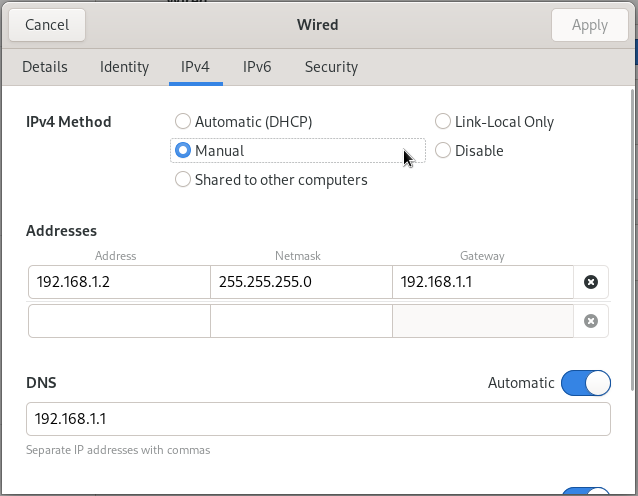
\includegraphics[width=\linewidth]{images/server-network-2.png}
              \caption{Cấu hình mạng máy Server (2)}
              \label{figure:server-network-2}
          \end{minipage}

    \item \textbf{Máy Desktop có cấu hình như sau:}
          \begin{itemize}
              \item Hệ điều hành: Lubuntu 22.04.3 LTS (Jammy Jellyfish)
              \item CPU: 1 Core \textit{(Hình \ref{figure:desktop-processor})}
              \item Ram: 4GB \textit{(Hình \ref{figure:desktop-ram})}
              \item Disk: 20GB \textit{(Hình \ref{figure:desktop-disk})}
              \item Network: NAT Network "QTHT" \textit{(Hình \ref{figure:desktop-network})}
          \end{itemize}

          \begin{minipage}
              {\linewidth}
              \captionsetup{type=figure}
              \centering
              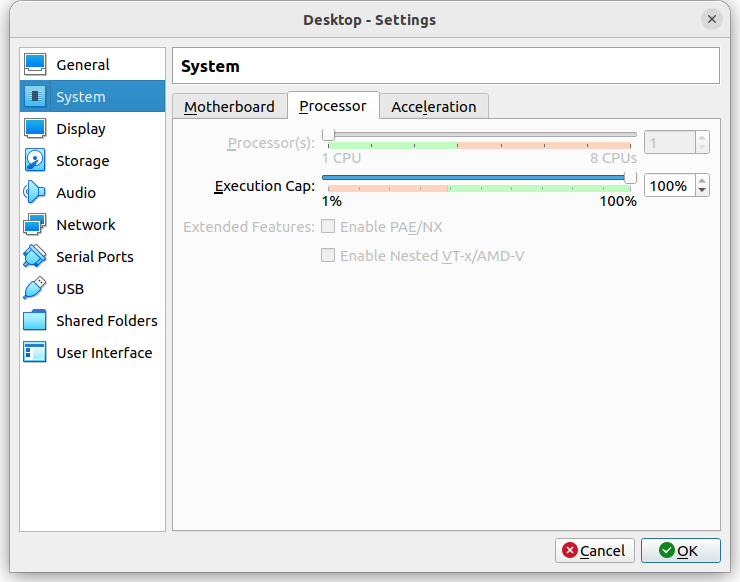
\includegraphics[width=\linewidth]{images/desktop-processor.png}
              \caption{Số Core CPU cho máy Desktop}
              \label{figure:desktop-processor}
          \end{minipage}

          \begin{minipage}
              {\linewidth}
              \captionsetup{type=figure}
              \centering
              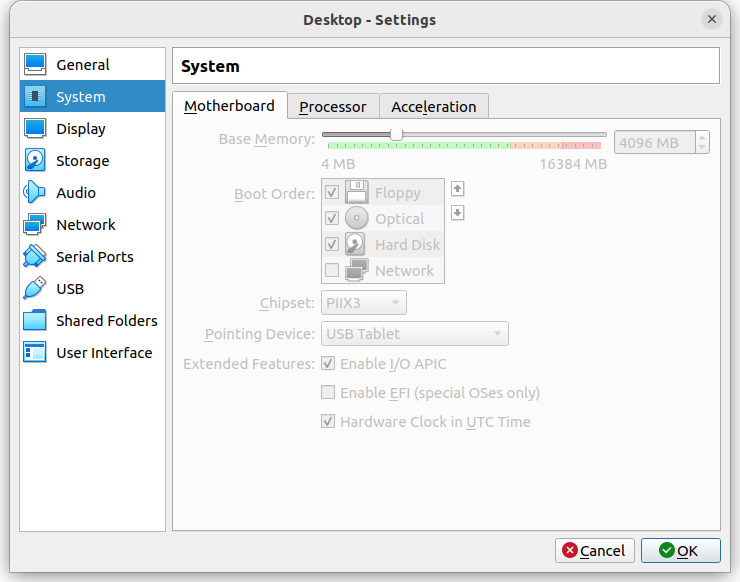
\includegraphics[width=\linewidth]{images/desktop-ram.png}
              \caption{Dung lượng RAM cho máy Desktop}
              \label{figure:desktop-ram}
          \end{minipage}

          \begin{minipage}
              {\linewidth}
              \captionsetup{type=figure}
              \centering
              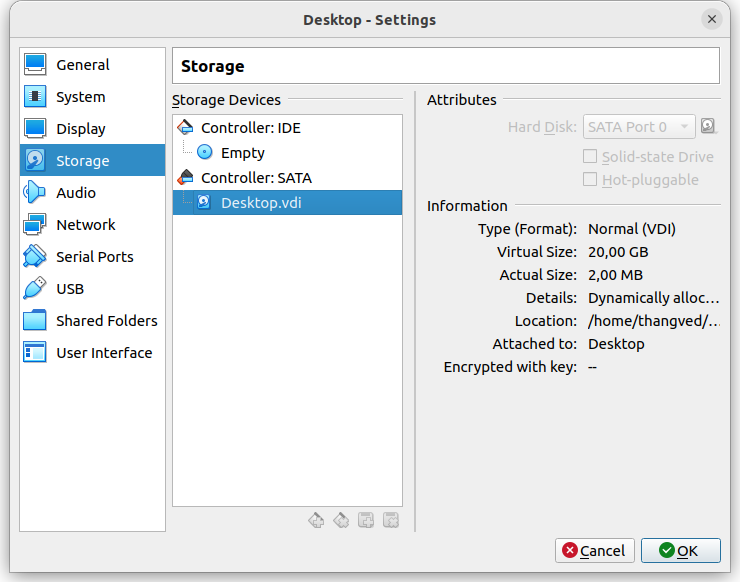
\includegraphics[width=\linewidth]{images/desktop-disk.png}
              \caption{Dung lượng ổ đĩa cho máy Desktop}
              \label{figure:desktop-disk}
          \end{minipage}

          \begin{minipage}
              {\linewidth}
              \captionsetup{type=figure}
              \centering
              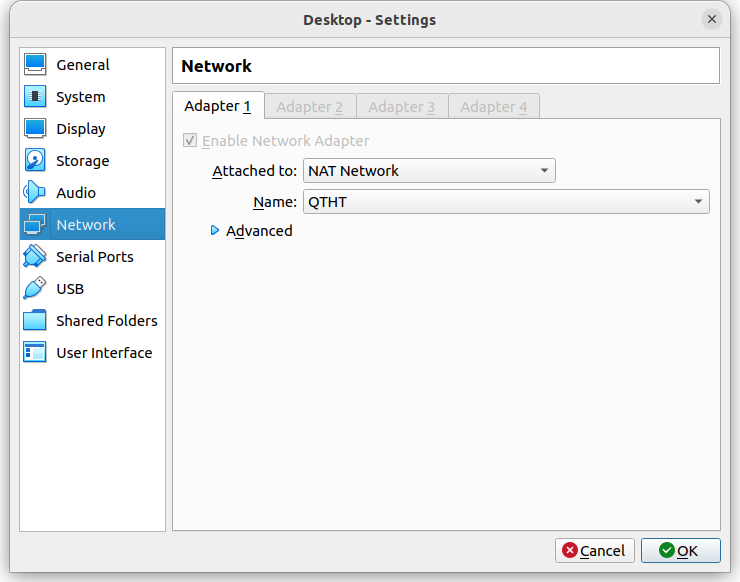
\includegraphics[width=\linewidth]{images/desktop-network.png}
              \caption{Cấu hình mạng cho máy Desktop}
              \label{figure:desktop-network}
          \end{minipage}
\end{enumerate}

\subsubsection{Tắt tường lửa trên máy Server}

Để tắt tường lửa ta có thể sử dụng lệnh \texttt{systemctl} hoặc \texttt{service}.
Ở đây ta sẽ sử dụng lệnh \texttt{systemctl} để làm việc này \textit{(xem Hình \ref{figure:stop-firewalld}) và Hình \ref{figure:disable-firewalld}}. \\

\begin{minipage}
    {\linewidth}
    \captionsetup{type=figure}
    \centering
    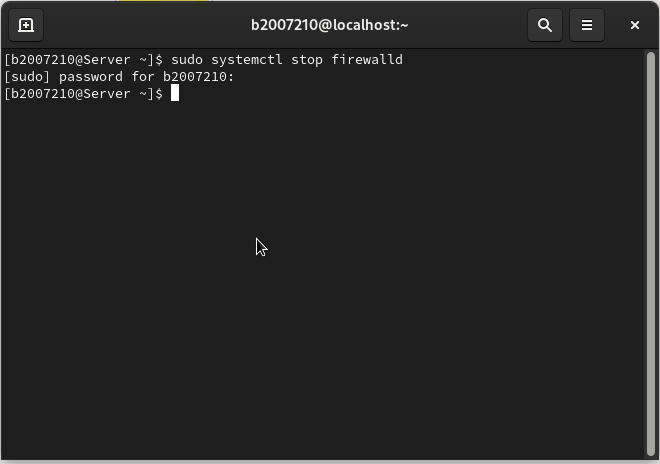
\includegraphics[width=\linewidth]{images/stop-firewalld.png}
    \caption{Dừng tường lửa bằng cách sử dụng \texttt{systemctl stop firewalld}}
    \label{figure:stop-firewalld}
\end{minipage}

\begin{lstlisting}[language=bash, caption=Dừng tường lửa]
sudo systemctl stop firewalld
\end{lstlisting}

\begin{minipage}
    {\linewidth}
    \captionsetup{type=figure}
    \centering
    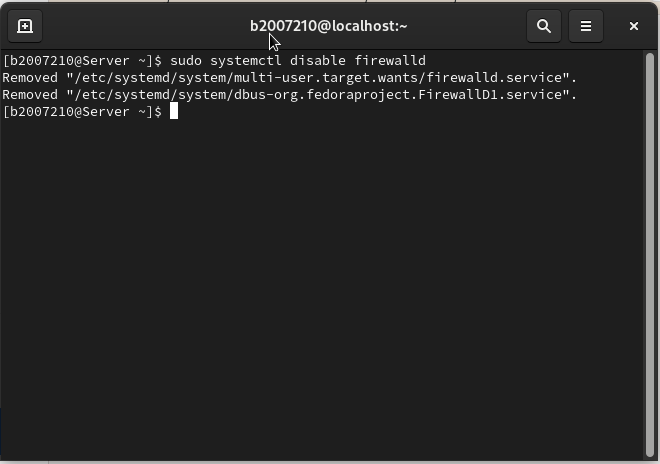
\includegraphics[width=\linewidth]{images/disable-firewalld.png}
    \caption{Ngăn tường lửa tự khởi động lại bằng cách sử dụng \texttt{systemctl disable firewalld}}
    \label{figure:disable-firewalld}
\end{minipage}

\begin{lstlisting}[language=bash, caption=Ngăn tường lửa tự khởi động lại]
sudo systemctl disable firewalld
\end{lstlisting}

Lệnh \texttt{systemctl stop firewalld} \textit{(Hình \ref{figure:stop-firewalld})} dùng để dừng tường lửa ngay lập tức và lệnh \texttt{systemctl disable firewalld} \textit{(Hình \ref{figure:disable-firewalld})} sẽ ngăn việc tường lửa tự khởi động lại sau khi reboot.

\subsection{(10\%) Tạo các người dùng và nhóm người dùng}

Để quản lý các bộ phận và người dùng trong công ty, hãy tạo các nhóm người dùng (group) và người dùng (user) trên server như sau. Cấp quyền sudo cho người dùng Nami.

\begin{longtable}{|c|c|c|c|c|c|}
    \caption{Danh sách người dùng và nhóm người dùng}              \\
    \hline
    STT & Họ tên  & Nhóm       & Username & Pasword & Mô tả        \\
    \hline

    1   & Luffy   & bangiamdoc & luffy    & luffy   & Giám đốc     \\
    \hline

    2   & Nami    & bangiamdoc & nami     & nami    & Phó giám đốc \\
    \hline

    3   & Zoro    & banhang    & zoro     & zoro    & Trưởng phòng \\
    \hline

    4   & Usopp   & banhang    & usopp    & usopp   & Nhân viên    \\
    \hline

    5   & Robin   & banhang    & robin    & robin   & Nhân viên    \\
    \hline

    6   & Sanji   & hanhchinh  & sanji    & sanji   & Trưởng phòng \\
    \hline

    7   & Chopper & hanhchinh  & chopper  & chopper & Nhân viên    \\
    \hline
\end{longtable}

\subsubsection{Tạo người dùng}

Để tạo người dùng trên CentOS, ta có thể sử dụng lệnh \texttt{useradd <username>} và dùng lệnh \texttt{passwd <username>} để đặt mật khẩu cho user.
Sau đây là ví dụ về việc tạo tài khoản và đặt mật khẩu cho tài khoản luffy \textit{(Hình \ref{figure:useradd-luffy})}.

\begin{minipage}
    {\linewidth}
    \captionsetup{type=figure}
    \centering
    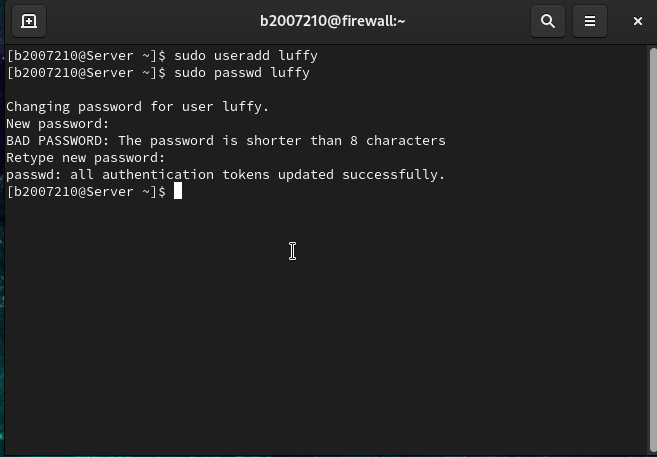
\includegraphics[width=\linewidth]{images/useradd-luffy.png}
    \caption{Tạo và đặt mật khẩu cho tài khoản luffy}
    \label{figure:useradd-luffy}
\end{minipage}

\begin{lstlisting}[language=bash, caption=Tạo và đặt mật khẩu cho tài khoản luffy]
sudo useradd luffy
sudo passwd luffy
\end{lstlisting}

Tương tự như thế với các tài khoản còn lại \textit{(Hình \ref{figure:useradd-other})}.

\begin{minipage}
    {\linewidth}
    \captionsetup{type=figure}
    \centering
    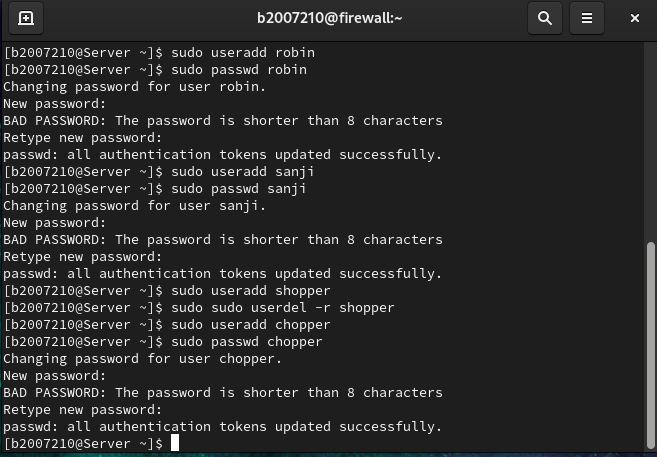
\includegraphics[width=\linewidth]{images/useradd-other.png}
    \caption{Tạo và đặt mật khẩu cho các người dùng còn lại}
    \label{figure:useradd-other}
\end{minipage}

\begin{lstlisting}[language=bash, caption=Tạo và đặt mật khẩu cho các người dùng còn lại]
sudo useradd nami
sudo passwd nami
sudo useradd zoro
sudo passwd zoro
sudo useradd usopp
sudo passwd usopp
sudo useradd robin
sudo passwd robin
sudo useradd sanji
sudo passwd sanji
sudo useradd chopper
sudo passwd chopper
\end{lstlisting}

\subsubsection{Tạo nhóm người dùng và thêm người dùng vào nhóm}

Để thêm nhóm người dùng, ta sử dụng lệnh \texttt{groupadd <group-name>} và thêm người dùng vào nhóm bằng lệnh \texttt{usermod -aG <group-name> <username>}.
Sau đây là ví dụ tạo nhóm \texttt{bangiamdoc} và thêm \texttt{luffy} và \texttt{nami} vào nhóm này \textit{(Hình \ref{figure:groupadd-bangiamdoc})}.

\begin{minipage}
    {\linewidth}
    \captionsetup{type=figure}
    \centering
    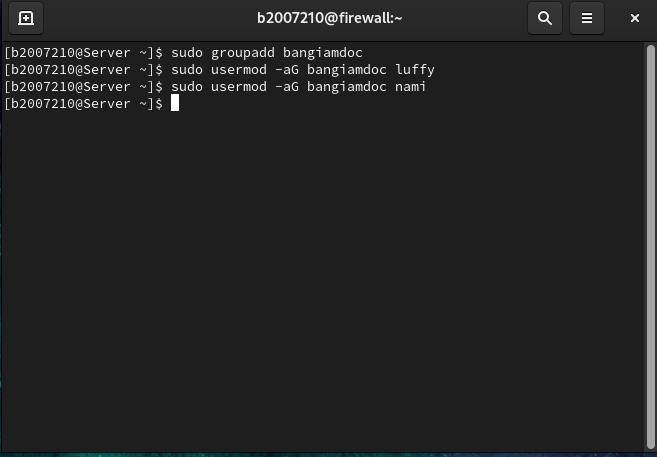
\includegraphics[width=\linewidth]{images/groupadd-bangiamdoc.png}
    \caption{Tạo nhóm bangiamdoc và thêm người dùng vào}
    \label{figure:groupadd-bangiamdoc}
\end{minipage}

\begin{lstlisting}[language=bash, caption=Tạo nhóm \texttt{bangiamdoc} và thêm người dùng vào]
sudo groupadd bangiamdoc
sudo usermod -aG bangiamdoc luffy
sudo usermod -aG bangiamdoc nami
\end{lstlisting}

Thực hiện tương tự với các nhóm còn lại \textit{(Hình \ref{figure:groupadd-other})}.

\begin{minipage}
    {\linewidth}
    \captionsetup{type=figure}
    \centering
    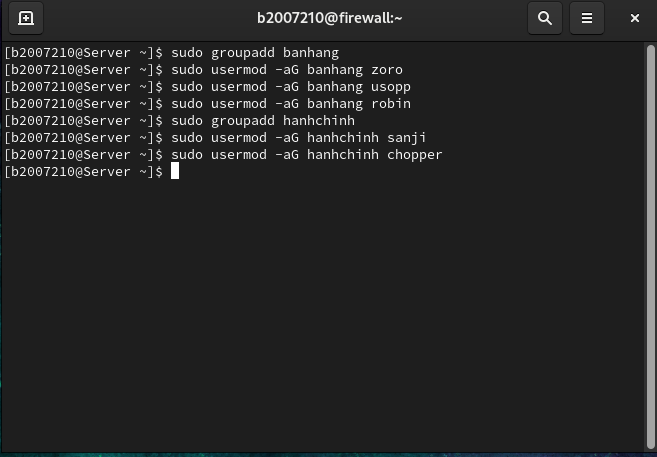
\includegraphics[width=\linewidth]{images/groupadd-other.png}
    \caption{Tạo các nhóm còn lại và thêm người dùng vào}
    \label{figure:groupadd-other}
\end{minipage}

\begin{lstlisting}[language=bash, caption=Tạo các nhóm còn lại và thêm người dùng vào]
sudo groupadd banhang
sudo usermod -aG banhang zoro
sudo usermod -aG banhang usopp
sudo usermod -aG banhang robin

sudo groupadd hanhchinh
sudo usermod -aG hanhchinh sanji
sudo usermod -aG hanhchinh chopper
\end{lstlisting}

\subsubsection{Cấp quyền sudo cho user nami}

Để cấp quyền sudo cho một user, ta chỉ cần thêm user đó vào nhóm \texttt{sudo} hoặc \texttt{wheel}.
Trong trường hợp này, ta sẽ thêm vào nhóm \texttt{wheel}.

\begin{minipage}
    {\linewidth}
    \captionsetup{type=figure}
    \centering
    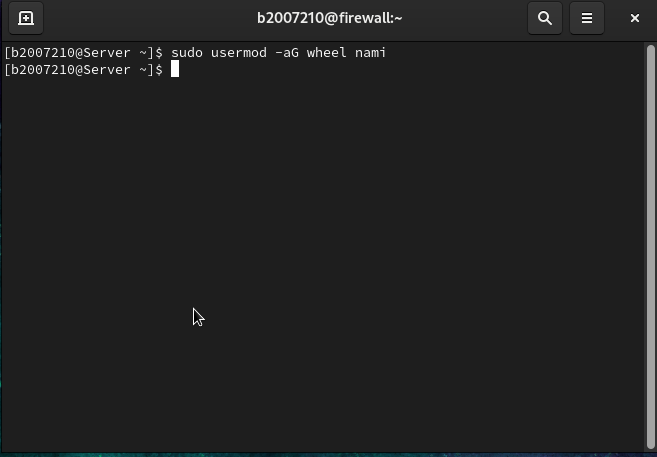
\includegraphics[width=\linewidth]{images/wheel-nami.png}
    \caption{Cấp quyền sudo cho user nami}
    \label{figure:wheel-nami}
\end{minipage}

\begin{lstlisting}[language=bash, caption=Cấp quyền sudo cho user nami]
sudo usermod -aG wheel nami
\end{lstlisting}

\subsection{(10\%)  Cài đặt và cấu hình dịch vụ SSH để cho phép điều khiển từ xa Server}

\begin{itemize}
    \item[--] Chỉ có thành viên ban giám đốc và tài khoản <Mã số sinh viên> mới có quyền điều khiển từ xa Server. Tài khoản root không được nối kết tới server từ xa.
    \item[--] Chỉ cho phép chứng thực bằng private key, không cho phép chứng thực bằng password. Tạo private/public key cho người dùng <Mã số sinh viên> để có thể SSH tới server.
\end{itemize}

\subsubsection{Cài đặt dịch vụ ssh}

\begin{minipage}
    {\linewidth}
    \captionsetup{type=figure}
    \centering
    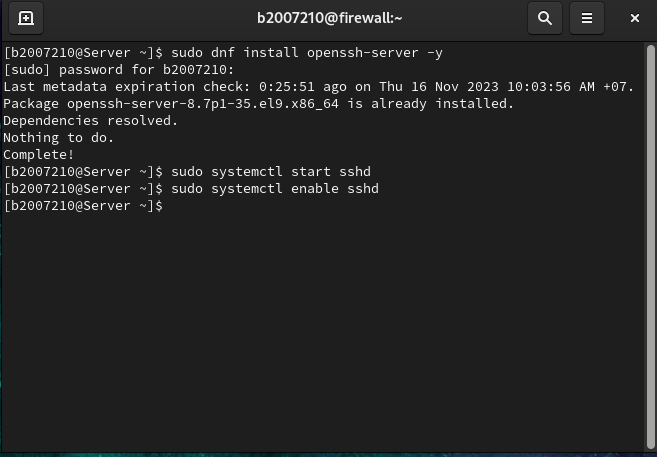
\includegraphics[width=\linewidth]{images/install-ssh.png}
    \caption{Cài đặt và kích hoạt dịch vụ ssh}
    \label{figure:install-ssh}
\end{minipage}
\begin{lstlisting}[language=bash, caption=Cài đặt và kích hoạt dịch vụ ssh]
sudo dnf install openssh-server
sudo systemctl enable sshd
sudo systemctl start sshd
\end{lstlisting}

\subsubsection{Cấu hình chỉ cho phép thành viên trong ban giám đốc và tài khoản \texttt{b2007210} mới có quyền điều khiển từ xa}

Để cấu hình chỉ cho phép một nhóm người dùng hoặc người dùng có thể sử dụng dịch vụ ssh, ta sẽ cấu hình trong file \texttt{/etc/ssh/sshd\_config} \textit{(Hình \ref{figure:allow-groups-users})}. \\
\begin{minipage}
    {\linewidth}
    \captionsetup{type=figure}
    \centering
    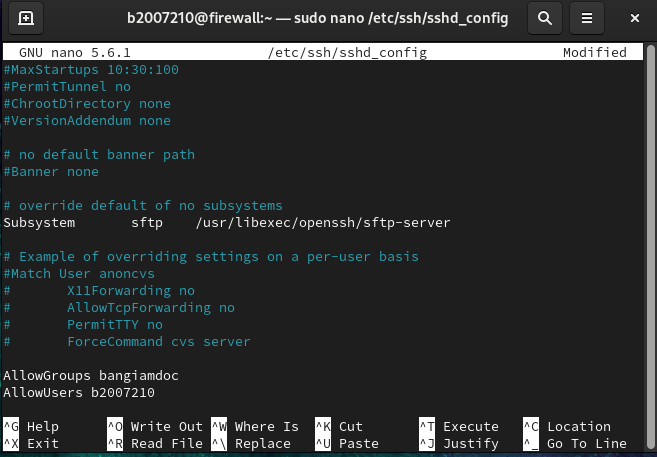
\includegraphics[width=\linewidth]{images/allow-groups-users.png}
    \caption{Cho phép nhóm \texttt{bangiamdoc} và user \texttt{b2007210} có quyền điều khiển máy tính từ xa}
    \label{figure:allow-groups-users}
\end{minipage}
\begin{itemize}
    \item[--] \texttt{AllowGroups bangiamdoc}: Cho phép nhóm \texttt{bangiamdoc} sử dụng dịch vụ ssh.
    \item[--] \texttt{AllowUsers b2007210}: Cho phép user \texttt{b2007210} sử dụng dịch vụ ssh.
\end{itemize}

Ta cần khởi động lại dịch vụ ssh để áp dụng những thay đổi này (dùng lệnh \texttt{systemctl restart sshd}).

\subsubsection{Chỉ cho phép chứng thực bằng private key}

Để cấu hình chỉ cho phép chứng thực bằng private key, ta sẽ cấu hình trong file \texttt{/etc/ssh/sshd\_config} \textit{(Hình \ref{figure:ssh-only-pubkey})}. \\
\begin{minipage}
    {\linewidth}
    \captionsetup{type=figure}
    \centering
    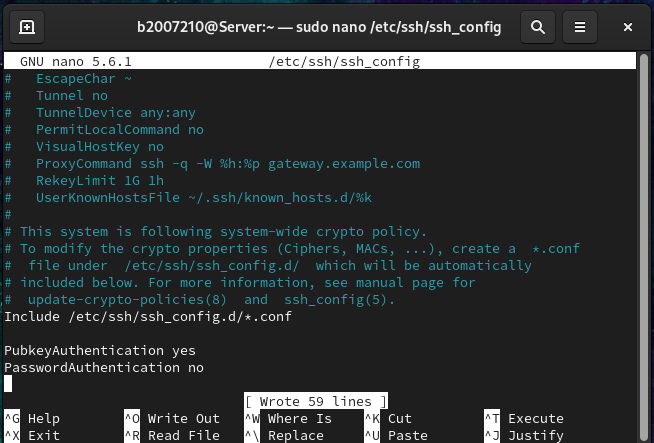
\includegraphics[width=\linewidth]{images/ssh-only-pubkey.png}
    \caption{Cấu hình cho phép truy cập dịch vụ ssh bằng private key}
    \label{figure:ssh-only-pubkey}
\end{minipage}
\begin{itemize}
    \item[--] \texttt{PubkeyAuthentication yes}: Cho phép chứng thực bằng private key.
    \item[--] \texttt{PasswordAuthentication no}: Không cho phép chứng thực bằng password.
\end{itemize}
Sau khi cấu hình xong, ta cần khởi động lại dịch vụ ssh để áp dụng những thay đổi này (dùng lệnh \texttt{systemctl restart sshd}).

Để tạo private key và public key, ta sử dụng lệnh \texttt{ssh-keygen} \textit{(Hình \ref{figure:ssh-keygen})}. \\
\begin{minipage}
    {\linewidth}
    \captionsetup{type=figure}
    \centering
    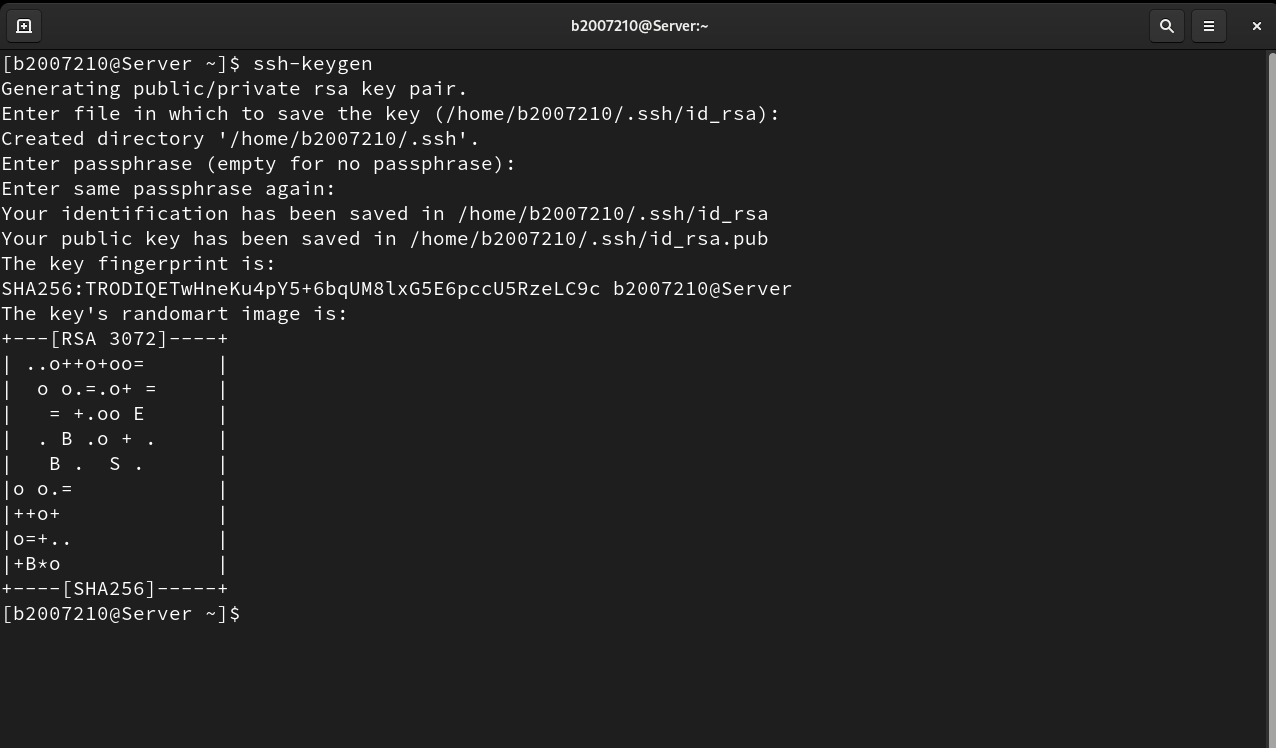
\includegraphics[width=\linewidth]{images/ssh-keygen.png}
    \caption{Tạo private key và public key}
    \label{figure:ssh-keygen}
\end{minipage}

Sau đó, ta cần đổi lại tên của public key thành \texttt{authorized\_keys} và phân lại quyền cho tập tin này \textit{(Hình \ref{figure:rename-authorized-keys})}. \\
\begin{minipage}
    {\linewidth}
    \captionsetup{type=figure}
    \centering
    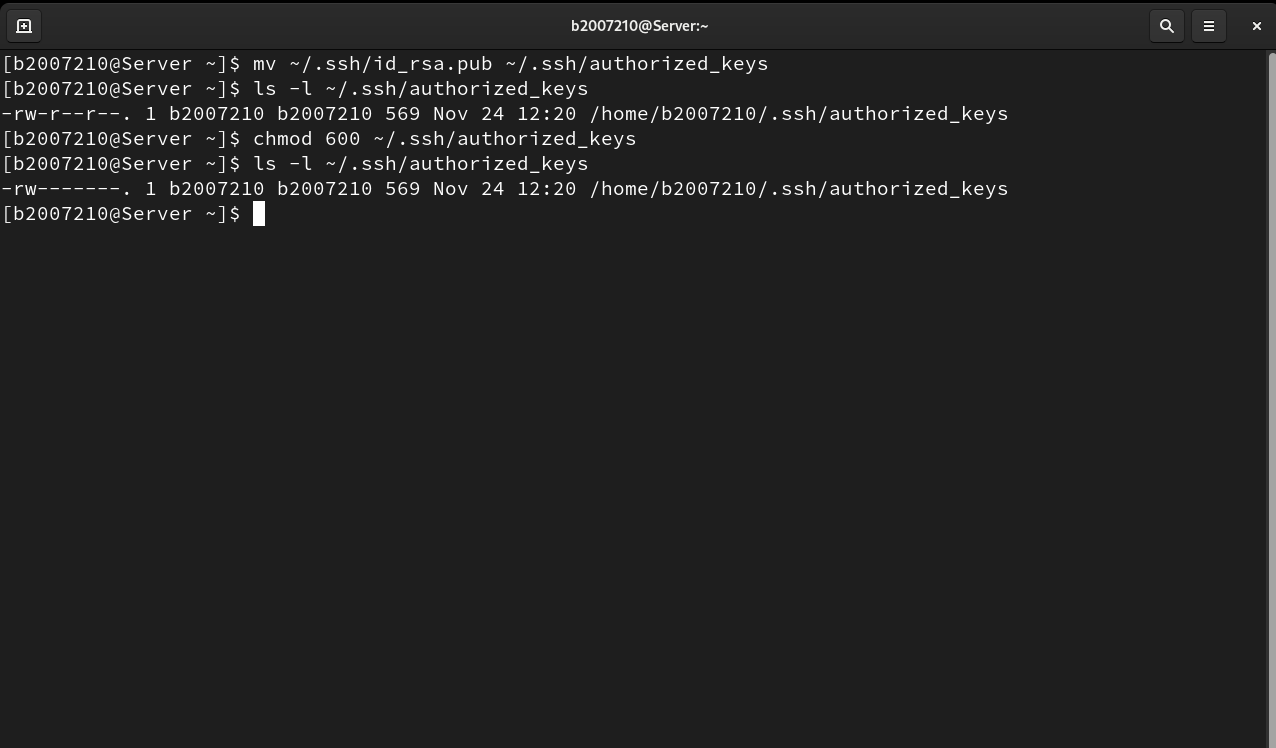
\includegraphics[width=\linewidth]{images/rename-authorized-keys.png}
    \caption{Đổi tên và phân quyền cho tập tin public key}
    \label{figure:rename-authorized-keys}
\end{minipage}

\begin{itemize}
    \item[--] Đổi tên tập tin public key thành \texttt{authorized\_keys}.
          \begin{lstlisting}[language=bash, caption=Đổi tên tập tin public key]
mv ~/.ssh/id\_rsa.pub ~/.ssh/authorized\_keys
\end{lstlisting}
    \item[--] Cho phép chủ sở hữu đọc và ghi vào tập tin \texttt{authorized\_keys}.
          \begin{lstlisting}[language=bash, caption=Phân quyền cho tập tin \texttt{authorized\_keys}]
chmod 600 ~/.ssh/authorized\_keys
\end{lstlisting}
\end{itemize}

\subsection{(10\%) Tạo và phân quyền cho thư mục \texttt{/data}}

Tạo thư mục /data trên server và phân quyền sao cho thành viên ban giám đốc có toàn quyền (read, write và execute), các trưởng phòng có quyền read và execute, các nhân viên không có bất cứ quyền gì. Ngoài ra chỉ chủ sở hữu tập tin có quyền xóa hoặc đổi tên tập tin trong thư mục /data.


Để tạo và phân quyền cho thư mục \texttt{/data}, ta thực hiện theo các bước như \textit{Hình \ref{figure:facl}}.

\begin{minipage}
    {\linewidth}
    \captionsetup{type=figure}
    \centering
    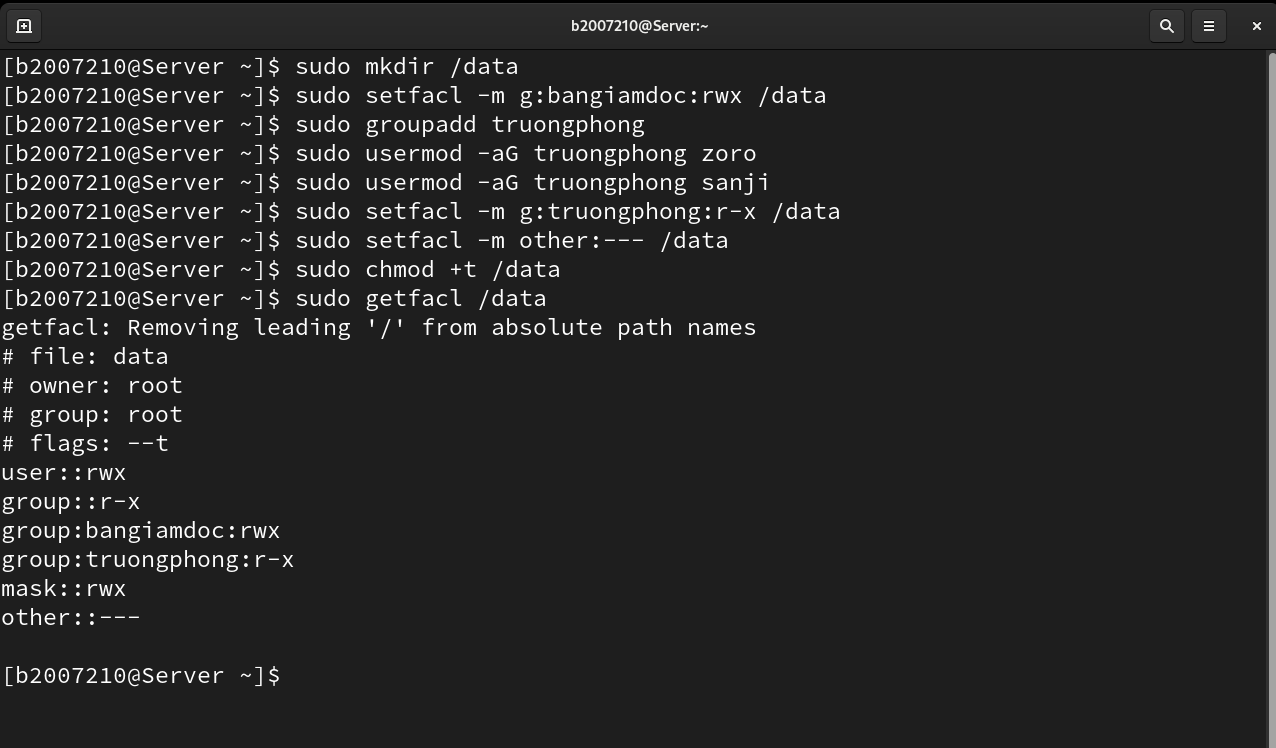
\includegraphics[width=\linewidth]{images/facl.png}
    \caption{Tạo và phân quyền cho thư mục \texttt{/data}}
    \label{figure:facl}
\end{minipage}

Cụ thể như sau:
\begin{enumerate}
    \item Tạo thư mục \texttt{/data}.
          \begin{lstlisting}[language=bash, caption=Tạo thư mục \texttt{/data}]
sudo mkdir /data
\end{lstlisting}
    \item Ban giám đốc có toàn quyền (read, write, execute) trên thư mục \texttt{/data}
          \begin{lstlisting}[language=bash, caption=Phân quyền cho ban giám đốc]
sudo setfacl -m g:bangiamdoc:rwx /data
\end{lstlisting}
    \item  Trưởng phòng có quyền read và execute trên thư mục \texttt{/data}
          \begin{lstlisting}[language=bash, caption=Phân quyền cho trưởng phòng]
sudo groupadd truongphong
sudo usermod -aG truongphong zoro
sudo usermod -aG truongphong sanji
sudo setfacl -m g:truongphong:rx /data
\end{lstlisting}

          \begin{itemize}
              \item [\textbf{Dòng 1}] Tạo nhóm \texttt{truongphong}.
              \item [\textbf{Dòng 2}] Thêm user \texttt{zoro} vào nhóm \texttt{truongphong}.
              \item [\textbf{Dòng 3}] Thêm user \texttt{sanji} vào nhóm \texttt{truongphong}.
              \item [\textbf{Dòng 4}] Phân quyền cho nhóm \texttt{truongphong} có quyền read và execute trên thư mục \texttt{/data}.
          \end{itemize}
    \item \textbf{Nhân viên} không có bất cứ quyền gì trên thư mục \texttt{/data}
          \begin{lstlisting}[language=bash, caption=Phân quyền cho nhân viên]
sudo setfacl -m other:--- /data
\end{lstlisting}
    \item Chỉ chủ sở hữu tập tin có quyền xóa hoặc đổi tên tập tin trong thư mục \texttt{/data}
          \begin{lstlisting}
sudo chmod +t /data
\end{lstlisting}
\end{enumerate}

\subsection{(5\%) Cài đặt và cấu hình tường lửa trên Server}

Có thể truy cập các dịch vụ DNS, DHCP, SSH, Web, SAMBA trên Server. Các dịch vụ khác KHÔNG cập truy cập được.

Ta sẽ cấu hình như \textit{Hình \ref{figure:config-firewall}}.

\begin{minipage}
    {\linewidth}
    \captionsetup{type=figure}
    \centering
    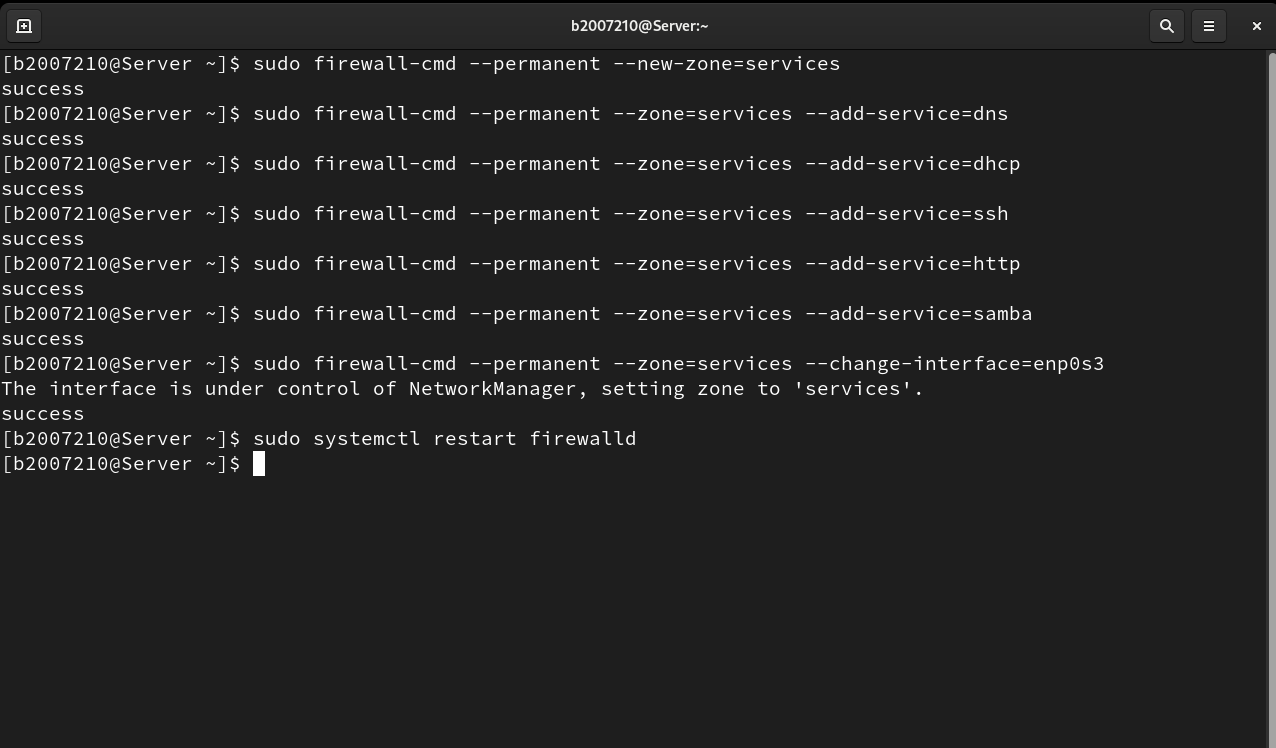
\includegraphics[width=\linewidth]{images/config-firewall.png}
    \caption{Cấu hình tường lửa trên Server}
    \label{figure:config-firewall}
\end{minipage}

Cụ thể như sau:
\begin{enumerate}
    \item Tạo một zone mới có tên là \texttt{services}
          \begin{lstlisting}[language=bash, caption=Tạo zone mới có tên là \texttt{services}]
sudo firewall-cmd --permanent --new-zone=services
\end{lstlisting}
    \item Thêm các dịch vụ DNS, DHCP, SSH, Web, SAMBA vào zone \texttt{services}
          \begin{lstlisting}[language=bash, caption={Thêm các dịch vụ DNS, DHCP, SSH, Web, SAMBA vào zone \texttt{services}}]
sudo firewall-cmd --permanent --zone=services --add-service=dns
sudo firewall-cmd --permanent --zone=services --add-service=dhcp
sudo firewall-cmd --permanent --zone=services --add-service=ssh
sudo firewall-cmd --permanent --zone=services --add-service=http
sudo firewall-cmd --permanent --zone=services --add-service=samba
\end{lstlisting}
    \item Khởi động lại dịch vụ tường lửa để áp dụng những thay đổi này
          \begin{lstlisting}
sudo systemctl restart firewalld
\end{lstlisting}
\end{enumerate}

\subsection{(5\%) Cài đặt và cấu hình dịch vụ DHCP trên Server để cấu hình mạng tự động cho các máy Desktop trong nhánh mạng}

\begin{itemize}
    \item[--] Địa chỉ IP của desktop: trong dãy 192.168.1.100/24 đến 192.168.1.254/24
    \item[--] Địa chỉ gateway:  192.168.1.1
    \item[--] DNS server: 192.168.1.2 và 8.8.8.8
\end{itemize}

\subsubsection{Cài đặt dịch vụ DHCP}

\begin{minipage}
    {\linewidth}
    \captionsetup{type=figure}
    \centering
    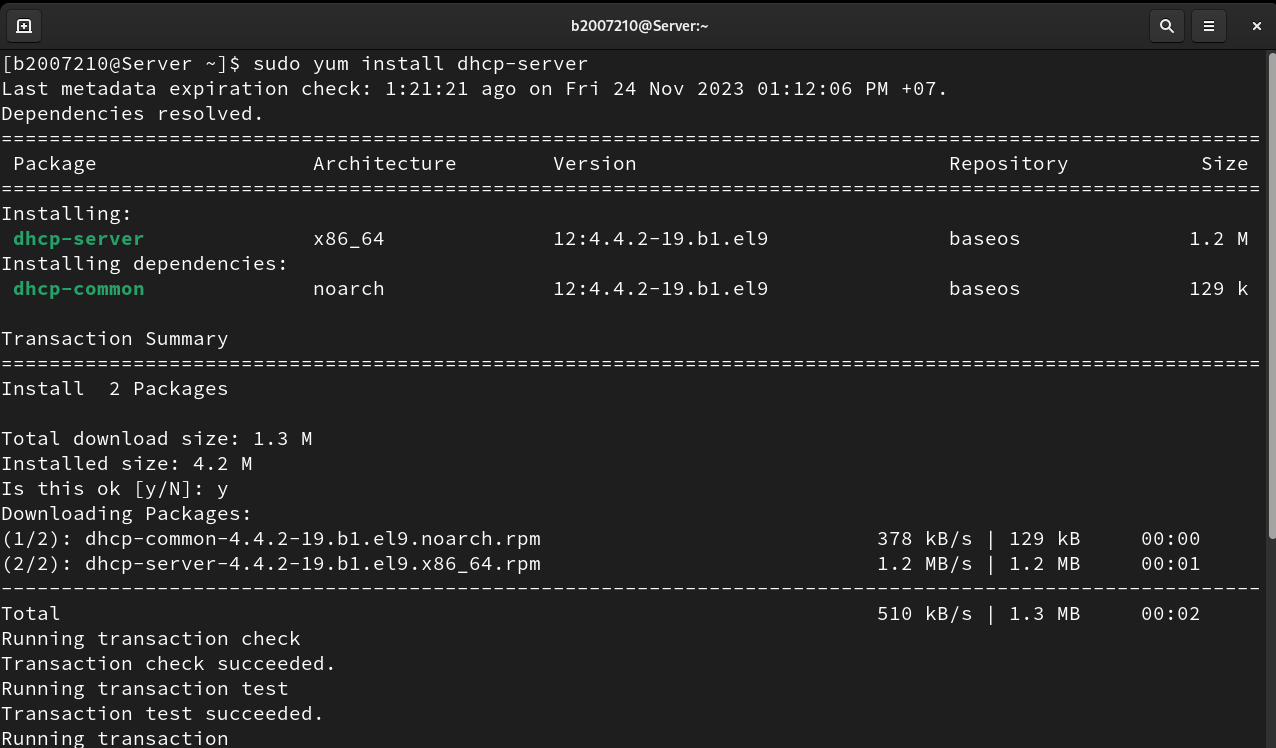
\includegraphics[width=\linewidth]{images/install-dhcp-server.png}
    \caption{Cài đặt dhcp-server}
    \label{figure:install-dhcp-server}
\end{minipage}
\begin{lstlisting}[language=bash, caption=Cài đặt dịch vụ DHCP]
sudo yum install dhcp-server
\end{lstlisting}

\subsubsection{Cấu hình dịch vụ dhcp}

Ta có thể cấu hình dịch vụ dhcp bằng cách chỉnh sửa nội dung file \texttt{/etc/dhcp/dhcpd.conf}

\begin{minipage}
    {\linewidth}
    \captionsetup{type=figure}
    \centering
    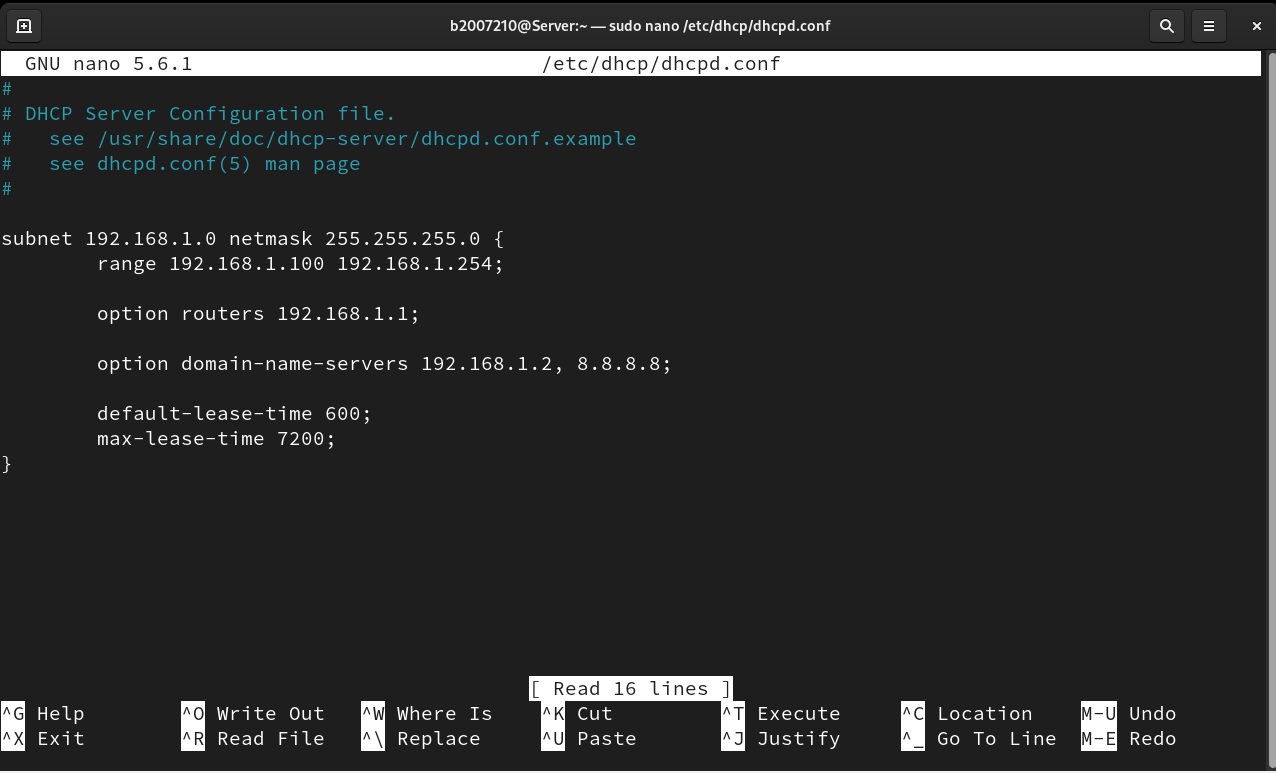
\includegraphics[width=\linewidth]{images/dhcpd-conf.png}
    \caption{Cấu hình dịch vụ dhcp}
    \label{figure:dhcpd-conf}
\end{minipage}
Nội dung file \texttt{/etc/dhcp/dhcpd.conf} như sau:
\begin{lstlisting}[language=bash, caption=Nội dung file \texttt{/etc/dhcp/dhcpd.conf}]
subnet 192.168.1.0 netmask 255.255.255.0 {
range 192.168.1.100 192.168.1.254;

option routers 192.168.1.1;

option domain-name-servers 192.168.1.2, 8.8.8.8;

default-lease-time 600;
max-lease-time 7200;
}
\end{lstlisting}
\begin{itemize}
    \item [\textbf{Dòng 1}] Cấu hình subnet là 255.255.255.0 với địa chỉ mạng là 192.168.1.0.
    \item [\textbf{Dòng 2}] Cấu hình range địa chỉ IP cho các máy desktop là từ 192.168.1.100 đến 192.168.1.254.
    \item [\textbf{Dòng 4}] Cấu hình địa chỉ gateway là 192.168.1.1.
    \item [\textbf{Dòng 6}] Cấu hình địa chỉ DNS server là
    \item [\textbf{Dòng 8}] Cấu hình thời gian mặc định mà một thiết bị sẽ được cấp phát địa chỉ IP là 600s.
    \item [\textbf{Dòng 9}] Cấu hình thời gian tối đa mà một thiết bị được cấp địa chỉ IP là 7200s (2h).
\end{itemize}

\subsubsection{Khởi động dịch vụ dhcp}

\begin{minipage}
    {\linewidth}
    \captionsetup{type=figure}
    \centering
    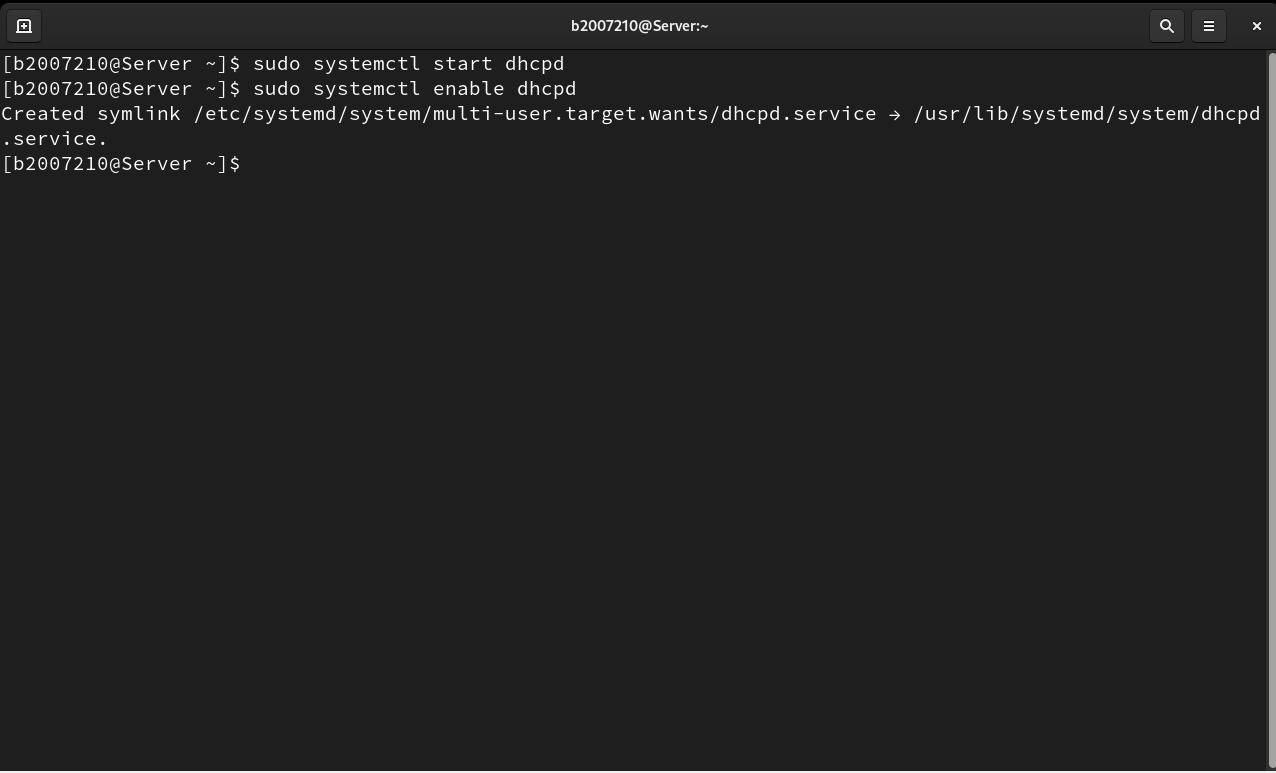
\includegraphics[width=\linewidth]{images/start-enable-dhcpd.png}
    \caption{Khởi động dịch vụ dhcp}
    \label{figure:start-enable-dhcpd}
\end{minipage}
\begin{lstlisting}[language=bash, caption=Khởi động dịch vụ dhcp]
sudo systemctl start dhcpd
sudo systemctl enable dhcpd
\end{lstlisting}

\subsubsection{Kiểm tra lại dịch vụ dhcp}

Sau khi cấu hình xong, ta sẽ kiểm tra lại bằng cách sử dụng máy desktop \textit{(Hình \ref{figure:desktop-ctu-thangved-com})} để kết nối vào mạng \texttt{QTHT} và kiểm tra địa chỉ IP của máy Desktop \textit{(Hình \ref{figure:desktop-ifconfig})}.

\begin{minipage}
    {\linewidth}
    \captionsetup{type=figure}
    \centering
    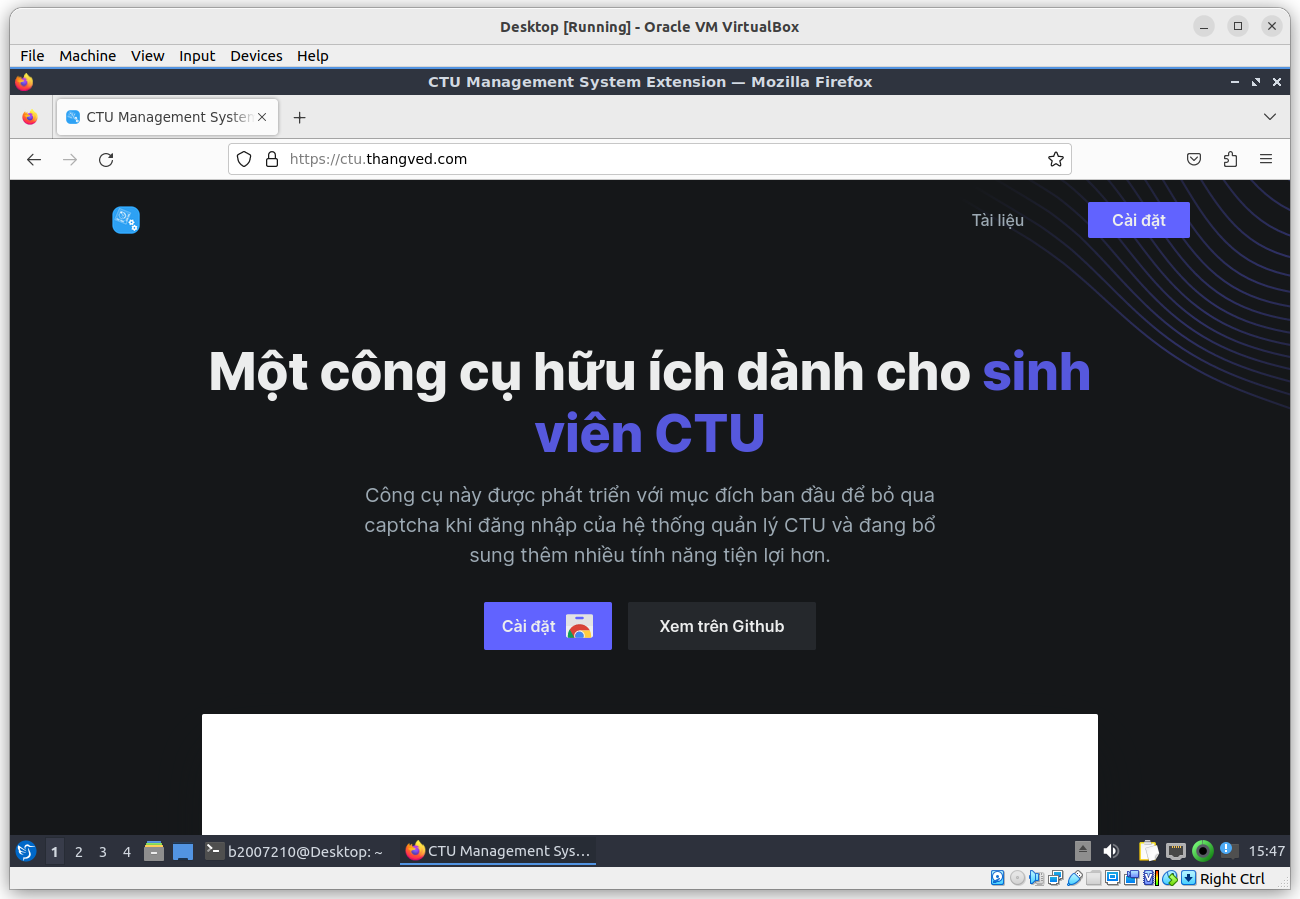
\includegraphics[width=\linewidth]{images/desktop-ctu-thangved-com.png}
    \caption{Truy cập vào internet bằng máy Desktop}
    \label{figure:desktop-ctu-thangved-com}
\end{minipage}

\begin{minipage}
    {\linewidth}
    \captionsetup{type=figure}
    \centering
    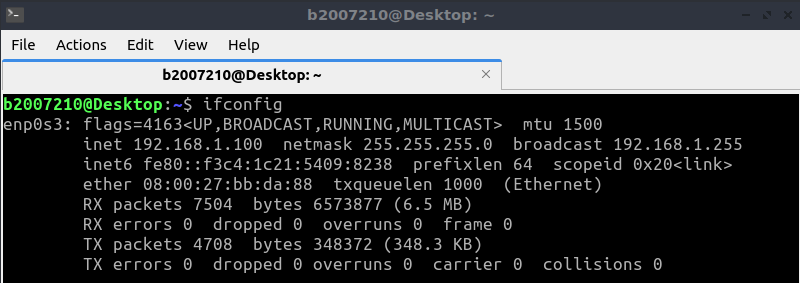
\includegraphics[width=\linewidth]{images/desktop-ifconfig.png}
    \caption{Kiểm tra địa chỉ IP của máy desktop (192.168.1.100)}
    \label{figure:desktop-ifconfig}
\end{minipage}

\subsection{(5\%) Cài đặt và cấu hình dịch vụ máy chủ Web trên Server sử dụng Docker}

Tạo một trang web cho công ty có tên miền strawhat.com với nội dung trang chủ giới thiệu về các thành viên trong công ty.

\subsubsection{Xây dựng trang web}

Có khá nhiều framework/thư viện hỗ trợ tạo trang web, ở đây ta sẽ sử dụng Vitejs để tạo một trang web đơn giản với thư viện Reactjs.
Mã nguồn trang web: \url{https://github.com/thangved/strawhat.com}

\begin{minipage}
    {\linewidth}
    \captionsetup{type=figure}
    \centering
    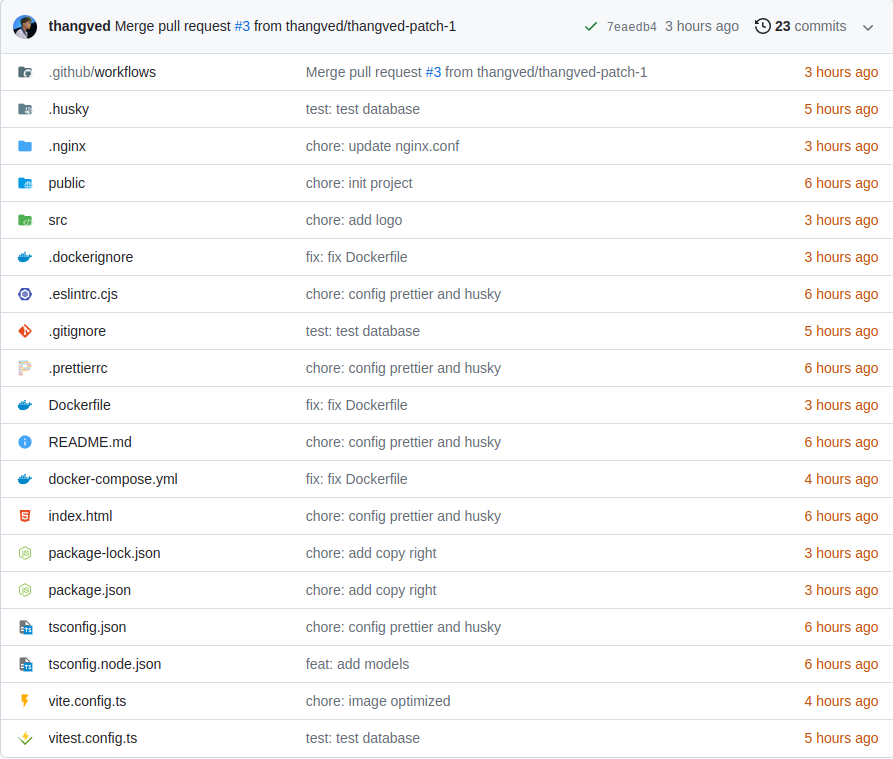
\includegraphics[width=\linewidth]{images/github-strawhat.png}
    \caption{Cấu trúc trang web strawhat.com}
    \label{figure:github-strawhat}
\end{minipage}

\subsubsection{Cấu hình Docker và nginx}
Ta cần quan tâm đến các file sau đây:
\begin{itemize}
    \item [--] \texttt{/Dockerfile} file này sẽ được sử dụng để build image cho container. \hfill
          \begin{lstlisting}[language=bash, caption={Nội dung file \texttt{/Dockerfile}}]
FROM node:20-alpine as development

WORKDIR /app

COPY package*.json .

RUN npm ci

COPY . .

CMD [ "npm", "run", "dev" ]

FROM development as production

RUN npm run build

FROM nginx:alpine

COPY --from=production /app/.nginx/nginx.conf /etc/nginx/conf.d/default.conf

WORKDIR /usr/share/nginx/html

RUN rm -rf ./*

COPY --from=production /app/dist .

ENTRYPOINT ["nginx", "-g", "daemon off;"]
\end{lstlisting}

          \begin{itemize}
              \item [\textbf{Dòng 1 - 11}] \textbf{Tạo môi trường phát triển bên trong docker container}
                    \begin{itemize}
                        \item [\texttt{1}] Sử dụng image \texttt{node:20-alpine} làm base image.
                        \item [\texttt{3}] Chỉ định thư mục làm việc bên trong image là /app.
                        \item [\texttt{5}] Sao chép tập tin package.json và package-lock.json vào bên trong image.
                        \item [\texttt{7}] Cài đặt các thư viện của dự án.
                        \item [\texttt{9}] Sao chép mã nguồn của dự án vào image.
                        \item [\texttt{11}] Lệnh npm run dev dùng để chạy dev server do Vitejs cấu hình.
                    \end{itemize}
              \item [\textbf{Dòng 13 - 15}] \textbf{Build bản production để triển khai}
                    \begin{itemize}
                        \item [\texttt{13}] Sử dụng image từ image development làm base image
                        \item [\texttt{15}] Lệnh \texttt{npm run dev} sẽ tạo một bản build của dự án này vào trong thư mục \texttt{dist}
                    \end{itemize}
              \item [\textbf{Dòng 17 - 27}] \textbf{Cấu hình nginx}
                    \begin{itemize}
                        \item [\texttt{17}] Sử dụng image \texttt{nginx:alpine} làm base image.
                        \item [\texttt{19}] Sao chép file cấu hình từ image production vào image và đổi tên thành /etc/nginx/conf.d/default.conf, đây là file config mặc định của nginx.
                        \item [\texttt{23}] Chỉ định thư mục làm việc.
                        \item [\texttt{23}] Xóa trang web mặc định của nginx.
                        \item [\texttt{25}] Sao chép bản dựng từ image production.
                        \item [\texttt{27}] Lệnh \texttt{nginx -g daemon off;} sẽ chạy nginx và không thoát ra.
                    \end{itemize}
          \end{itemize}

    \item [--] \texttt{/docker-compose.yml}. \hfill
          \begin{lstlisting}[language=bash, caption={Nội dung file \texttt{/docker-compose.up}}]
version: '3.7'

services:
    strawhat.com:
        build: .
        container_name: strawhat.com
        ports:
            - '80:80'
\end{lstlisting}
          \begin{itemize}
              \item [\textbf{Dòng 1}] Sử dụng phiên bản 3.7 của docker-compose.
              \item [\textbf{Dòng 3}] Tạo một service có tên là \texttt{strawhat.com}.
              \item [\textbf{Dòng 4}] Sử dụng Dockerfile để build image cho service này.
              \item [\textbf{Dòng 5}] Đặt tên cho container là \texttt{strawhat.com}.
              \item [\textbf{Dòng 6}] Chỉ định cổng 80 của máy host sẽ được map vào cổng 80 của container.
          \end{itemize}
    \item [--] \texttt{/.nginx/nginx.conf} file này sẽ được sử dụng để cấu hình nginx. \hfill
          \begin{lstlisting}[language=bash, caption={Nội dung file \texttt{/.nginx/nginx.conf}}]
server {
    server_name strawhat.com www.strawhat.com;

    listen 80;

    location / {
        root /usr/share/nginx/html;
        index index.html index.htm;
        try_files $uri /index.html =404;
    }

    error_page 500 502 503 504 /50x.html;

    location = /50x.html {
        root /usr/share/nginx/html;
    }
}
\end{lstlisting}
          \begin{itemize}
              \item [\textbf{Dòng 2}] Cấu hình server name là strawhat.com và www.strawhat.com, khi một request có domain là strawhat.com hoặc www.strawhat.com được gửi đến server này, nginx sẽ xử lý request này.
              \item [\textbf{Dòng 4}] Cấu hình nginx lắng nghe trên cổng 80.
              \item [\textbf{Dòng 6}] Cấu hình thư mục root là /usr/share/nginx/html.
              \item [\textbf{Dòng 7}] Cấu hình file index mặc định là index.html.
              \item [\textbf{Dòng 8}] Cấu hình thử các file tĩnh nếu không tìm thấy file index.html, do đây là trang web SPA nên ta sẽ thử các file tĩnh trước khi trả về trang index.html.
              \item [\textbf{Dòng 10}] Cấu hình trang 50x.html.
              \item [\textbf{Dòng 12}] Cấu hình thư mục root cho trang 50x.html.
              \item [\textbf{Dòng 14}] Cấu hình trang 50x.html.
              \item [\textbf{Dòng 16}] Cấu hình thư mục root cho trang 50x.html.
          \end{itemize}

\end{itemize}

\subsubsection{Chạy trang web trên máy host}

Để chạy thử web trên máy host, ta sẽ dùng lệnh \texttt{docker compose up} để docker sẽ tự động kéo các image trên cloud và build image cho service \texttt{strawhat.com} sau đó chạy container từ image này.

\begin{minipage}
    {\linewidth}
    \captionsetup{type=figure}
    \centering
    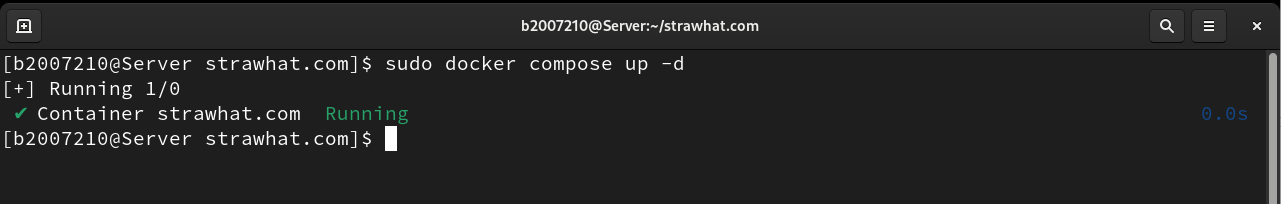
\includegraphics[width=\linewidth]{images/run-webserver.png}
    \caption{Chạy trang web bằng lệnh \texttt{docker compose up}}
    \label{figure:run-webserver}
\end{minipage}

Lúc này, trang web sẽ được chạy trên cổng 80 của máy host như đã cấu hình trong file \texttt{docker-compose.yml} \textit{(Hình \ref{figure:run-webserver})}.

\begin{minipage}
    {\linewidth}
    \captionsetup{type=figure}
    \centering
    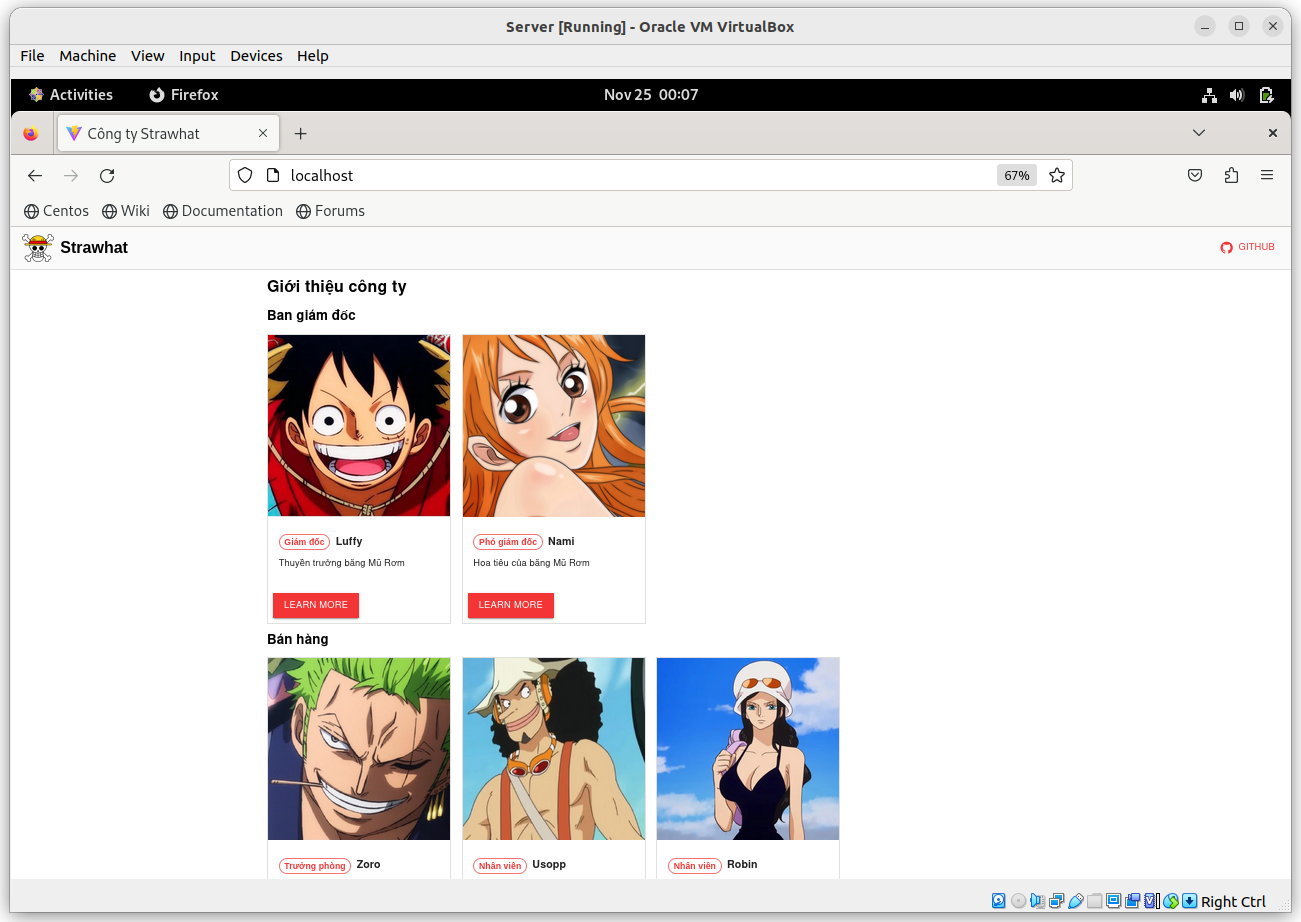
\includegraphics[width=\linewidth]{images/strawhat-localhost.png}
    \caption{Giao diện trang web strawhat.com}
    \label{figure:strawhat-localhost}
\end{minipage}

Ta có thể thử chỉnh sửa DNS của máy host để trỏ tên miền strawhat.com về địa chỉ localhost để kiểm tra trang web đã hoạt động chính xác hay chưa.

\begin{minipage}
    {\linewidth}
    \captionsetup{type=figure}
    \centering
    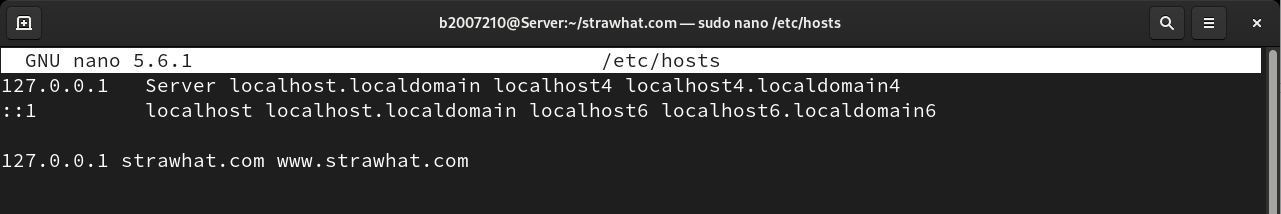
\includegraphics[width=\linewidth]{images/edit-etc-hosts.png}
    \caption{Chỉnh sửa file \texttt{/etc/hosts} để trỏ tên miền strawhat.com về địa chỉ localhost}
    \label{figure:edit-etc-hosts}
\end{minipage}

Sau khi cấu hình xong, ta có thể truy cập vào trang web theo địa chỉ \texttt{http://strawhat.com} \textit{(Hình \ref{figure:server-strawhat-com})}.

\begin{minipage}
    {\linewidth}
    \captionsetup{type=figure}
    \centering
    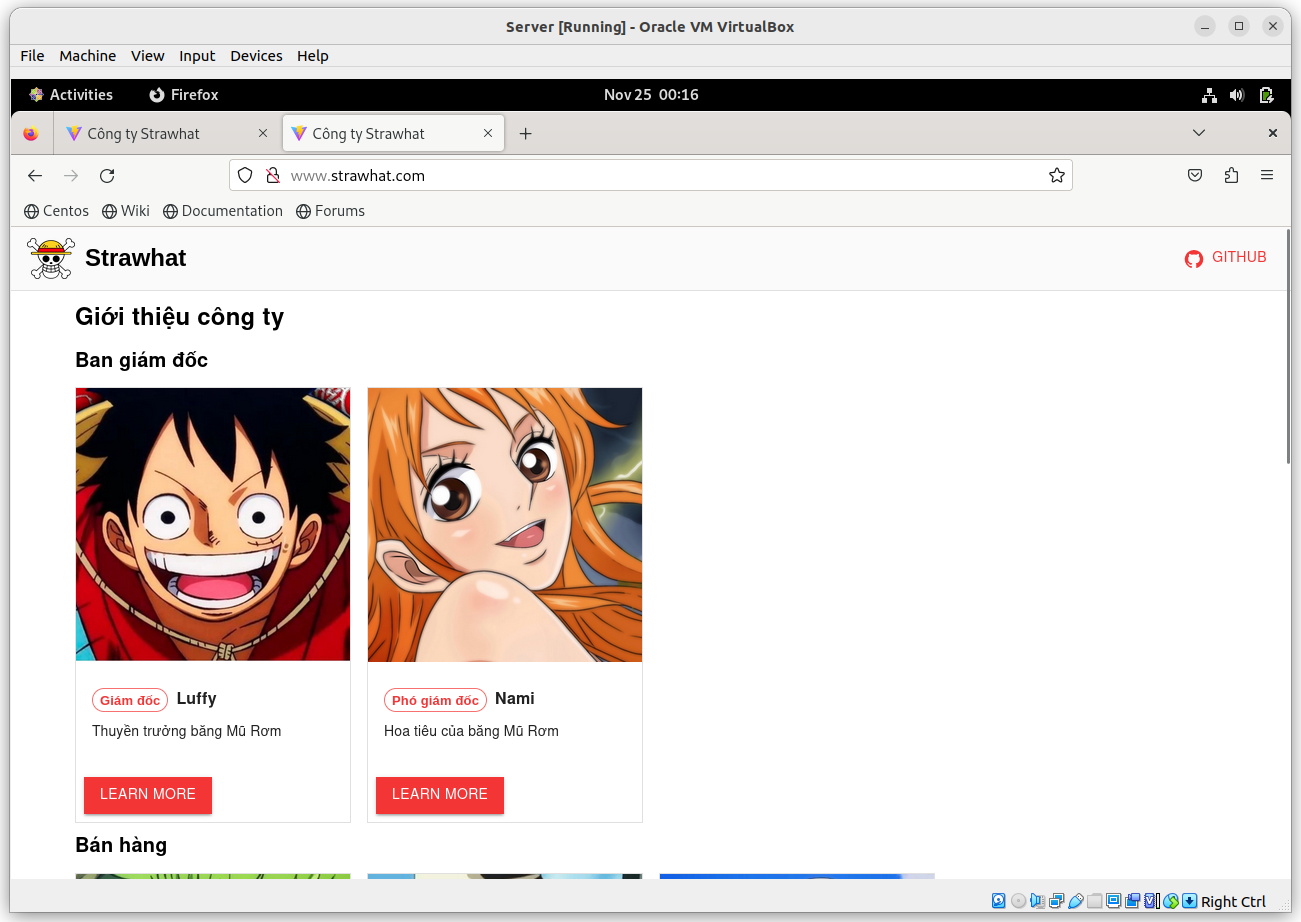
\includegraphics[width=\linewidth]{images/server-strawhat-com.png}
    \caption{Truy cập vào trang web từ server qua địa chỉ \texttt{http://strawhat.com}}
    \label{figure:server-strawhat-com}
\end{minipage}

\subsection{(5\%) Cài đặt và cấu hình dịch vụ SAMBA trên Server}

\begin{itemize}
    \item[--] Thành viên ban giám đốc và trưởng phòng có thể truy cập vào thư mục /data trên Server.
    \item[--] Tất cả người dùng có thể truy cập vào thư mục cá nhân của họ (/home/<username>) trên Server.
    \item[--] Trên Desktop tạo ổ cứng ảo nối kết tới dịch vụ SAMBA trên Server.
\end{itemize}

\subsubsection{Cài đặt dịch vụ SAMBA}

Để cài đặt dịch vụ SAMBA, ta sử dụng lệnh \texttt{sudo dnf install samba}.
Sau đó, ta tiến hành cấu hình dịch vụ trong file /etc/samba/smb.conf như sau:

\subsubsection{Thành viên ban giám đốc và trưởng phòng có thể truy cập vào thư mục /data trên Server}

Ta thực hiện cấu hình quyền truy cập vào thư mục /data như \textit{Hình \ref{figure:samba-config-data}}.

\begin{minipage}
    {\linewidth}
    \captionsetup{type=figure}
    \centering
    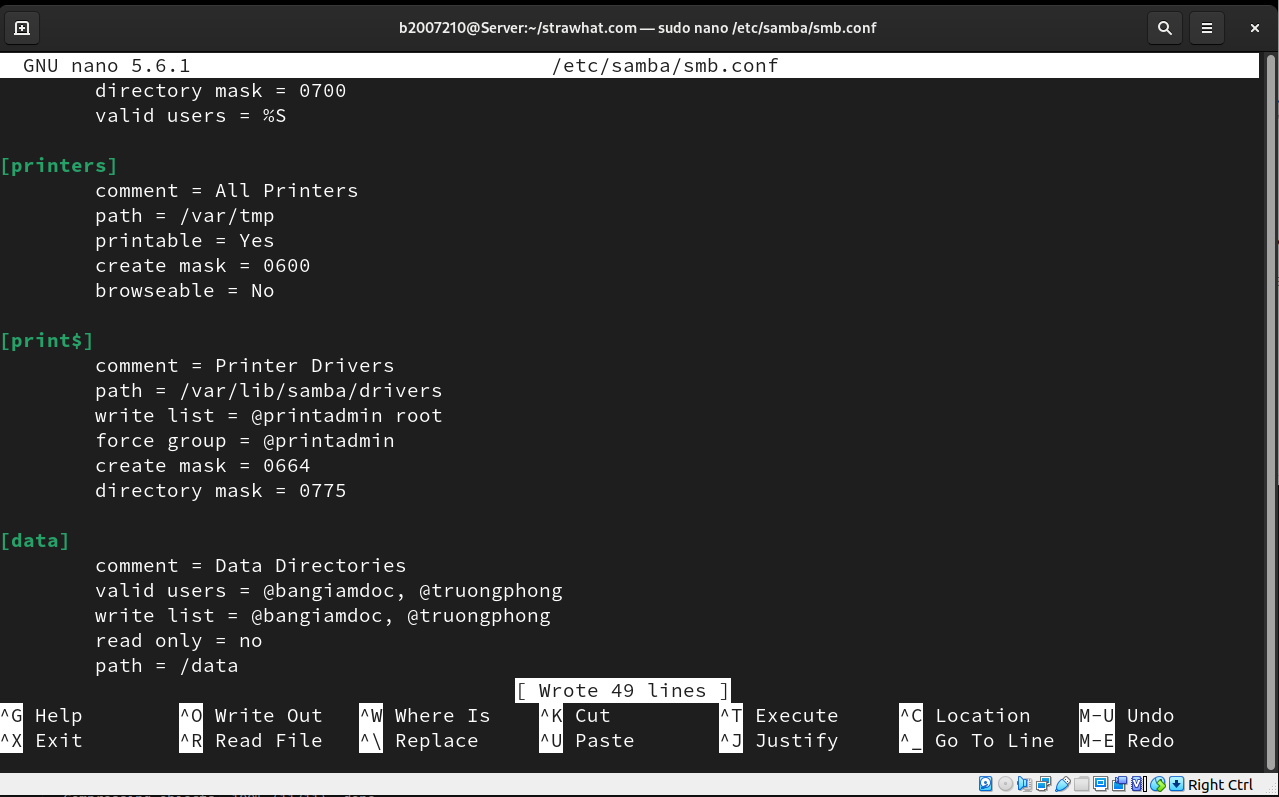
\includegraphics[width=\linewidth]{images/samba-config-data.png}
    \caption{Cấu hình quyền truy cập vào thư mục /data trên Server}
    \label{figure:samba-config-data}
\end{minipage}

\begin{lstlisting}[language=bash, caption=Cấu hình quyền truy cập vào thư mục /data trên Server]
[data]
    path = /data
    valid users = @bangiamdoc, @truongphong
    write list = @bangiamdoc, @truongphong
    read only = no
\end{lstlisting}

\begin{itemize}
    \item[\textbf{Dòng 2}] Chỉ định đường dẫn của thư mục.
    \item[\textbf{Dòng 3}] Danh sách những người dùng được quyền truy cập.
    \item[\textbf{Dòng 4}] Danh sách người dùng có quyền ghi dữ liệu vào thư mục.
    \item[\textbf{Dòng 5}] \texttt{read only} đặt thành \texttt{no} để cho phép ghi dữ liệu vào thư mục.
\end{itemize}


\subsubsection{Tất cả người dùng có thể truy cập vào thư mục cá nhân của họ (/home/<username>) trên Server}

Ta thực hiện cấu hình quyền truy cập vào thư mục cá nhân của người dùng như \textit{Hình \ref{figure:samba-config-homes}}.

\begin{minipage}
    {\linewidth}
    \captionsetup{type=figure}
    \centering
    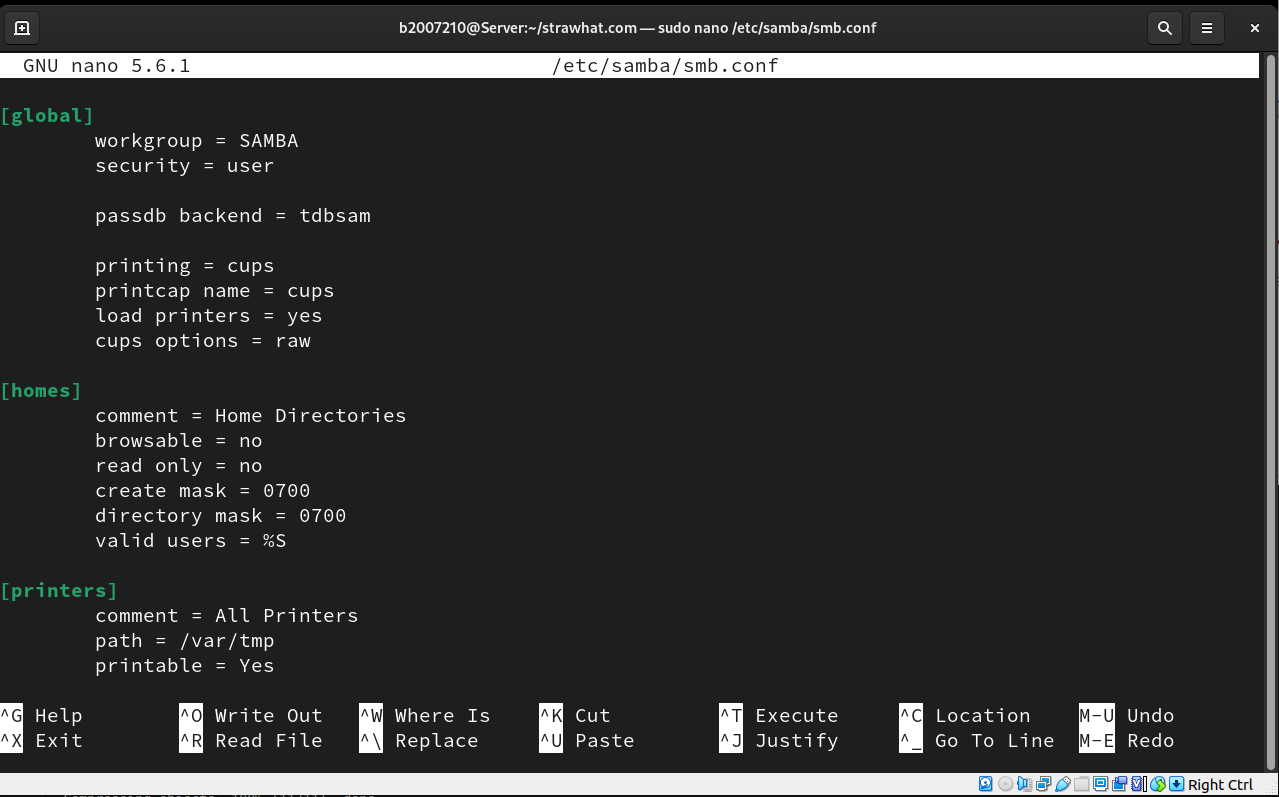
\includegraphics[width=\linewidth]{images/samba-config-homes.png}
    \caption{Cấu hình quyền truy cập vào thư mục /home/<username> trên Server}
    \label{figure:samba-config-homes}
\end{minipage}

\begin{lstlisting}[language=bash, caption=Cấu hình quyền truy cập vào thư mục /home/<username> trên Server]
[homes]
    comment = Home Directories
    browseable = no
    read only = no
    create mask = 0700
    directory mask = 0700
    valid users = %S
\end{lstlisting}

\begin{itemize}
    \item [\textbf{Dòng 2}] Chỉ định đường dẫn của thư mục.
    \item [\textbf{Dòng 3}] \texttt{browseable} đặt thành \texttt{no} để không hiển thị thư mục này.
    \item [\textbf{Dòng 4}] \texttt{read only} đặt thành \texttt{no} để cho phép ghi dữ liệu vào thư mục.
    \item [\textbf{Dòng 5}] \texttt{create mask} đặt thành \texttt{0700} để chỉ cho phép chủ sở hữu có quyền đọc, ghi và thực thi.
    \item [\textbf{Dòng 6}] \texttt{directory mask} đặt thành \texttt{0700} để chỉ cho phép chủ sở hữu có quyền đọc, ghi và thực thi.
    \item [\textbf{Dòng 7}] \texttt{valid users} đặt thành \texttt{\%S} để chỉ cho phép chủ sở hữu có quyền đọc, ghi và thực thi.
\end{itemize}

Sau đó, ta cần tạo mật khẩu dịch vụ samba cho các tài khoản bằng lệnh \texttt{smbpasswd -a <user-name>}.

\begin{minipage}
    {\linewidth}
    \captionsetup{type=figure}
    \centering
    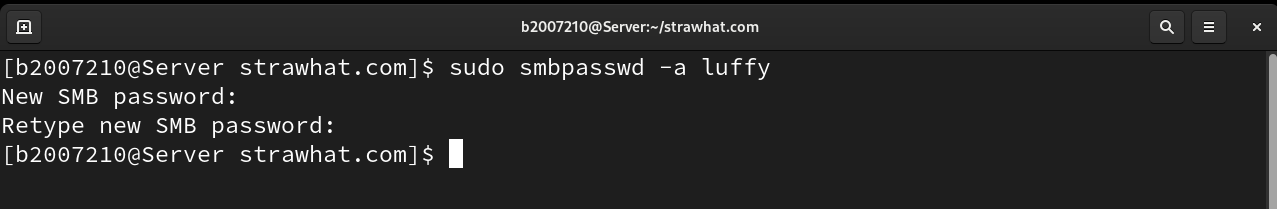
\includegraphics[width=\linewidth]{images/smb-passwd-luffy.png}
    \caption{Đặt mật khẩu dịch vụ samba cho tài khoản luffy}
    \label{figure:smb-passwd-luffy}
\end{minipage}

\begin{lstlisting}[language=bash, caption={Đặt mật khẩu dịch vụ samba cho tài khoản luffy}]
sudo smbpasswd -a luffy
\end{lstlisting}

Cuối cùng, ta cần khởi động lại dịch vụ samba để áp dụng thay đổi.

\begin{lstlisting}[language=bash, caption={Khởi động lại dịch vụ samba}]
sudo systemctl restart smb
\end{lstlisting}

\subsubsection{Trên Desktop tạo ổ cứng ảo nối kết tới dịch vụ SAMBA trên Server}

Ta có thể kết nối tới dịch vụ samba từ máy Desktop bằng cách sử dụng File Manager \textit{(Hình \ref{figure:samba-desktop})}.

\begin{minipage}
    {\linewidth}
    \captionsetup{type=figure}
    \centering
    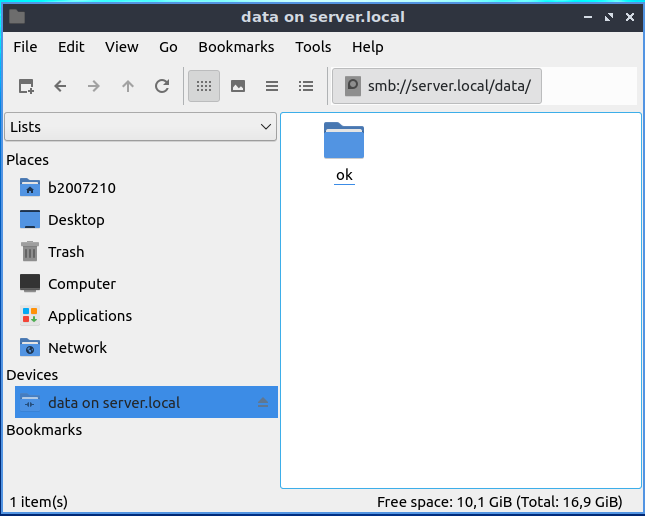
\includegraphics[width=\linewidth]{images/samba-desktop.png}
    \caption{Truy cập dịch vụ samba từ máy Desktop}
    \label{figure:samba-desktop}
\end{minipage}

Ta có thể kiểm tra dịch vụ samba đã hoạt động đúng hay chưa bằng cách tạo một file trên máy Desktop và xem trên Server đã được tạo hay chưa.

\begin{multicols}{2}
    \begin{minipage}
        {\linewidth}
        \captionsetup{type=figure}
        \centering
        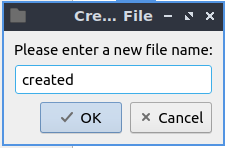
\includegraphics[width=\linewidth]{images/samba-created.png}
        \caption{Kiểm tra tạo file bằng dịch vụ samba (máy Desktop)}
        \label{figure:samba-created}
    \end{minipage}

    \begin{minipage}
        {\linewidth}
        \captionsetup{type=figure}
        \centering
        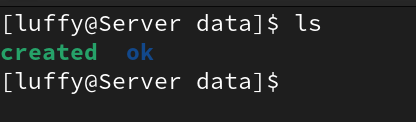
\includegraphics[width=\linewidth]{images/samba-created-server.png}
        \caption{Kiểm tra tạo file bằng dịch vụ samba (máy Server)}
        \label{figure:samba-created-server}
    \end{minipage}
\end{multicols}

\subsection{(5\%) Cài đặt và cấu hình dịch vụ DNS trên Server để phân giải tên miền strawhat.com}

\begin{itemize}
    \item[--] Tên miền: \url{www.strawhat.com} <----> IP: 192.168.1.2 (Server IP)
    \item[--] Tên miền: \url{gateway.strawhat.com} <----> IP: 192.168.1.1
\end{itemize}

\subsubsection{Cài đặt dịch vụ DNS}

Để cài đặt dịch vụ DNS, ta sử dụng lệnh \texttt{sudo dnf install bind bind-utils}.

\subsubsection{Cấu hình máy chủ DNS trên máy Server}

\begin{minipage}
    {\linewidth}
    \captionsetup{type=figure}
    \centering
    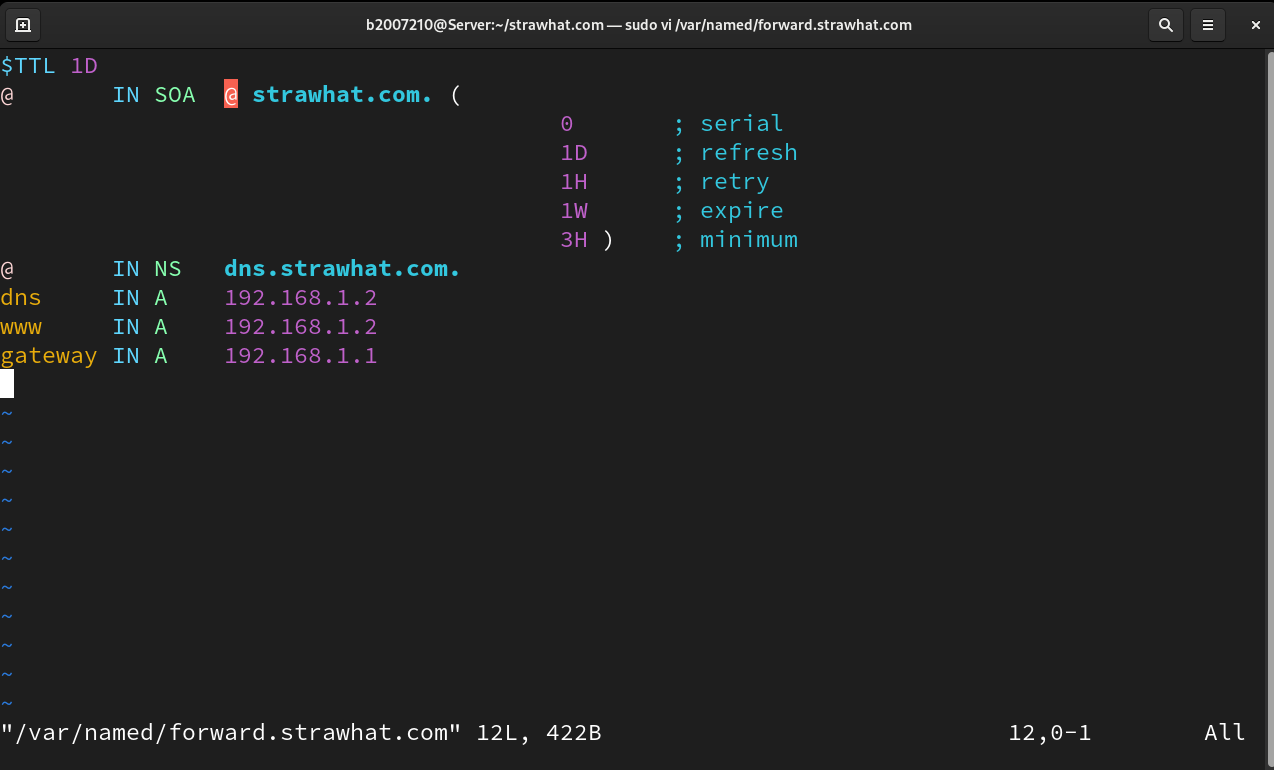
\includegraphics[width=\linewidth]{images/forward-strawhat-com.png}
    \caption{Nội dung file /var/named/forward.strawhat.com}
    \label{figure:forward-strawhat-com}
\end{minipage}

\begin{lstlisting}[language=bash, caption={Nội dung file /var/named/forward.strawhat.com}]
$TTL 1D
@       IN SOA      @       strawhat.com. (
                                0       ; serial
                                1D      ; refresh
                                1H      ; retry
                                1W      ; expire
                                3H )    ; minimum
@       IN NS       dns.strawhat.com.
@       IN A        192.168.1.2
www     IN A        192.168.1.2
gateway IN A        192.168.1.1
\end{lstlisting}

\begin{minipage}
    {\linewidth}
    \captionsetup{type=figure}
    \centering
    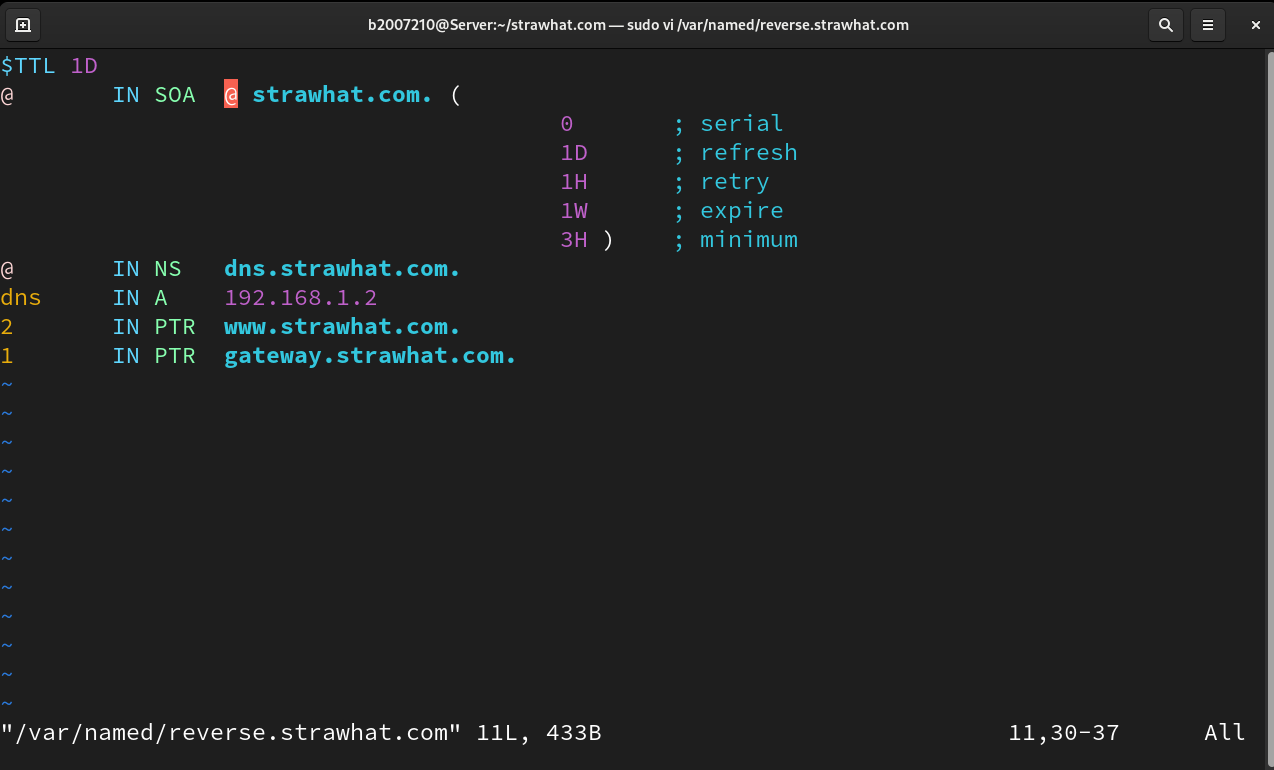
\includegraphics[width=\linewidth]{images/reverse-strawhat-com.png}
    \caption{Nội dung file /var/named/reverse.strawhat.com}
    \label{figure:reverse-strawhat-com}
\end{minipage}

\begin{lstlisting}[language=bash, caption={Nội dung file /var/named/reverse.strawhat.com}]
$TTL 1D
@       IN SOA      @       strawhat.com. (
                                0       ; serial
                                1D      ; refresh
                                1H      ; retry
                                1W      ; expire
                                3H )    ; minimum

@       IN NS       dns.strawhat.com.
dns     IN A        192.168.1.2
2       IN PTR      dns.strawhat.com.
1       IN PTR      gateway.strawhat.com.
\end{lstlisting}

\begin{minipage}
    {\linewidth}
    \captionsetup{type=figure}
    \centering
    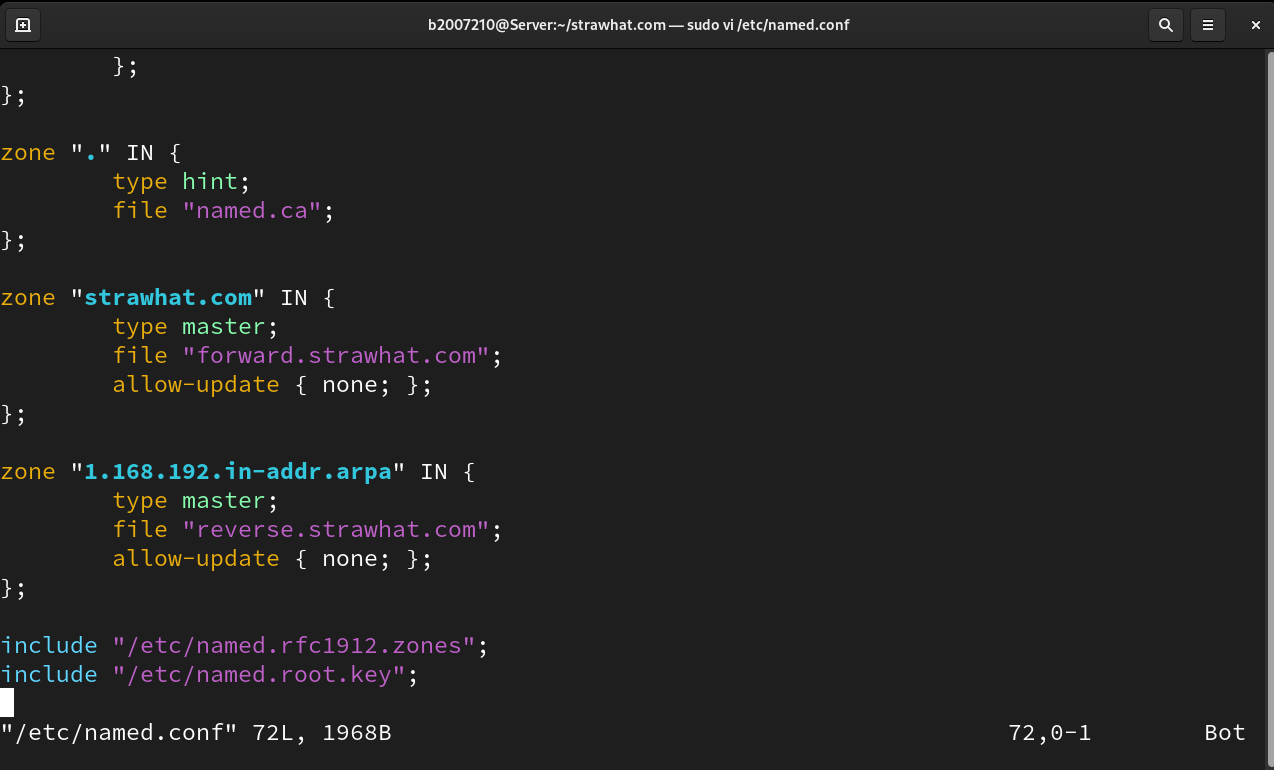
\includegraphics[width=\linewidth]{images/named-conf.png}
    \caption{Nội dung file /etc/named.conf}
    \label{figure:named-conf}
\end{minipage}

\begin{lstlisting}[language=bash, caption={Nội dung file /etc/named.conf}]
...

zone "." IN {
    ...
};

zone "strawhat.com" IN {
    type master;
    file "forward.strawhat.com";
    allow-update { none; };
};

zone "1.168.192.in-addr.arpa" IN {
    type master;
    file "reverse.strawhat.com";
    allow-update { none; };
};

...
\end{lstlisting}

\subsubsection{Khởi động dịch vụ DNS}

Ta cần khởi động dịch vụ DNS để áp dụng thay đổi.

\begin{lstlisting}[language=bash, caption={Khởi động dịch vụ DNS}]
sudo systemctl restart named
sudo systemctl enable named
\end{lstlisting}

\subsubsection{Kiểm tra trên máy Desktop}

Ta sử dụng máy Desktop để kiểm tra xem máy chủ DNS đã được cấu hình đúng hay chưa \textit{(Hình \ref{figure:test-dns-desktop})}.

\begin{minipage}
    {\linewidth}
    \captionsetup{type=figure}
    \centering
    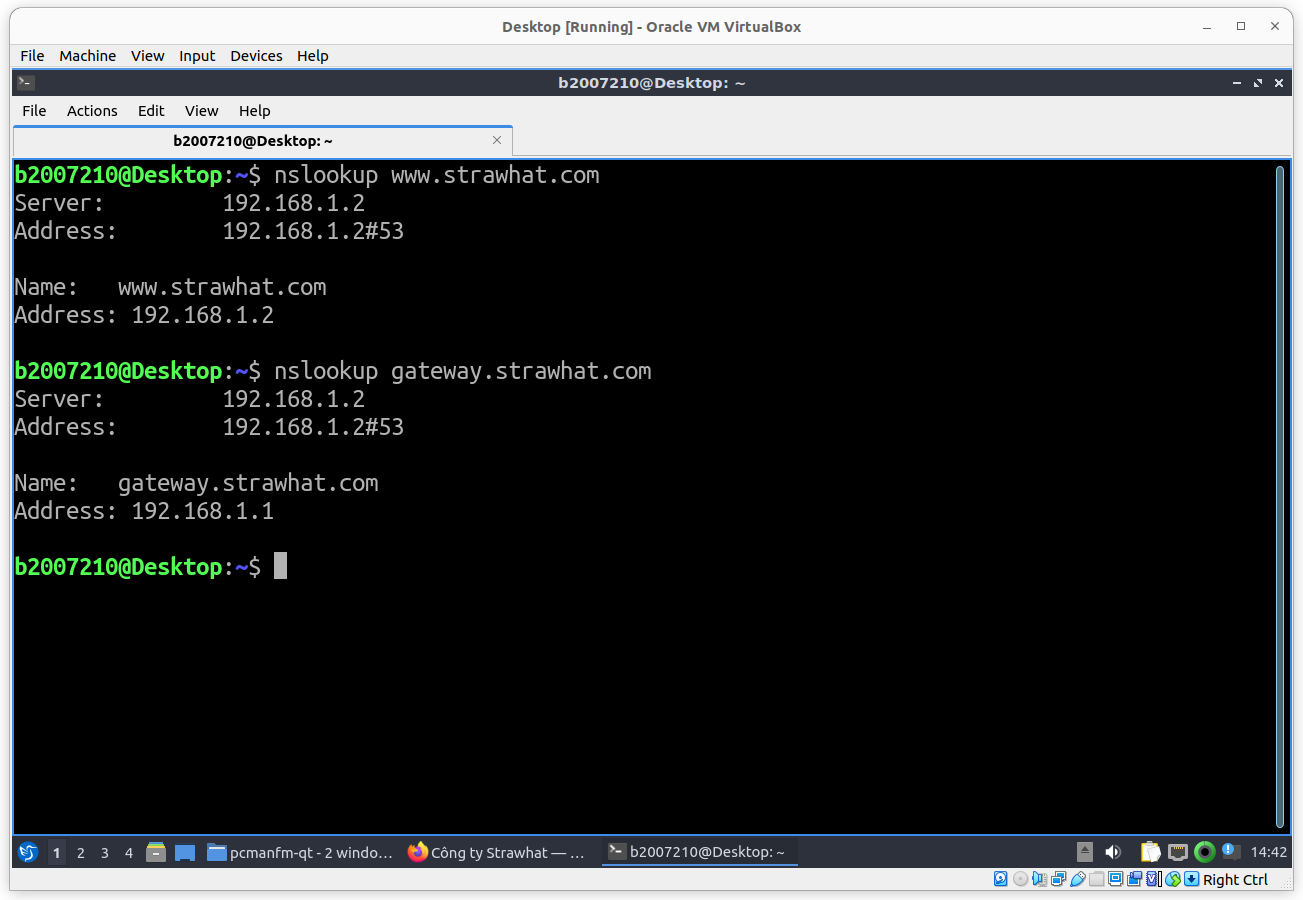
\includegraphics[width=\linewidth]{images/test-dns-desktop.png}
    \caption{Kiểm tra DNS trên máy Desktop}
    \label{figure:test-dns-desktop}
\end{minipage}

\subsection{(5\%) Sử dụng dịch vụ cron và shell script tự động thực hiện công việc sao lưu dữ liệu mỗi ngày, mỗi tuần, mỗi tháng trên Server}

\begin{itemize}
    \item[--] Các thư mục cần sao lưu sao lưu: /home, /data, /etc.
    \item[--] Nơi lưu dữ liệu sao lưu: /mnt/backup.
    \item[--] Sao lưu mỗi ngày: thực hiện vào lúc 23:59 từ thứ 2 đến thứ 7, dữ liệu sẽ được nén lại và lưu với tên như sau: backup\_<thứ> (ví dụ: backup\_monday).
    \item[--] Sao lưu mỗi tuần: thực hiện vào lúc 23:59 ngày chủ nhật hàng tuần, dữ liệu sẽ được nén lại và lưu với tên như sau: backup\_week<thứ tự tuần> (ví dụ: backup\_week1).
    \item[--] Sao lưu mỗi tháng: thực hiện vào lúc 23:59 ngày 1 hằng tháng, dữ liệu sẽ được nén lại và lưu với tên backup\_month1 nếu là tháng lẻ, backup\_month2 nếu là tháng chẵn.
\end{itemize}

\subsubsection{Tạo thư mục sao lưu dữ liệu}

Ta sẽ tạo thư mục \texttt{/mnt/backup} để lưu trữ dữ liệu sao lưu.

\begin{lstlisting}[language=bash, caption={Tạo thư mục sao lưu dữ liệu}]
sudo mkdir /mnt/backup
\end{lstlisting}

\subsubsection{Viết script backup}

Ta sẽ viết một script để thực hiện sao lưu dữ liệu theo các bước sau:
\begin{itemize}
    \item[--] Tạo một biến lưu trữ tên file theo yêu cầu
    \item[--] Nén các thư mục /home /data /etc
\end{itemize}

\begin{minipage}
    {\linewidth}
    \captionsetup{type=figure}
    \centering
    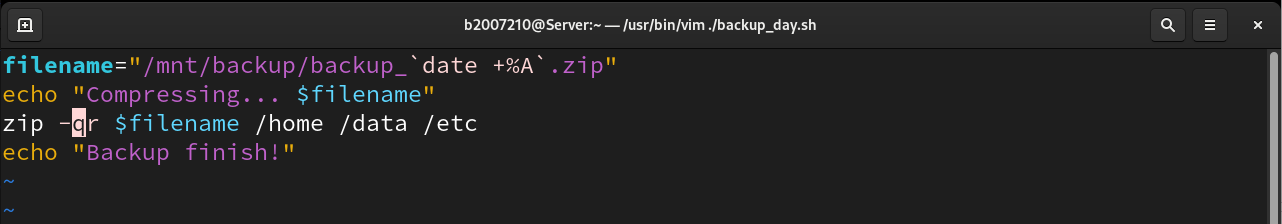
\includegraphics[width=\linewidth]{images/backup_day.png}
    \caption{Script backup mỗi ngày}
    \label{figure:backup_day}
\end{minipage}

\begin{lstlisting}[language=bash, caption={Script backup mỗi ngày}]
filename="/mnt/backup/backup_$(date +%A).zip"
echo "Compressing... $filename"
zip -qr $filename /home /data /etc
echo "Backup finish!"
\end{lstlisting}


\begin{minipage}
    {\linewidth}
    \captionsetup{type=figure}
    \centering
    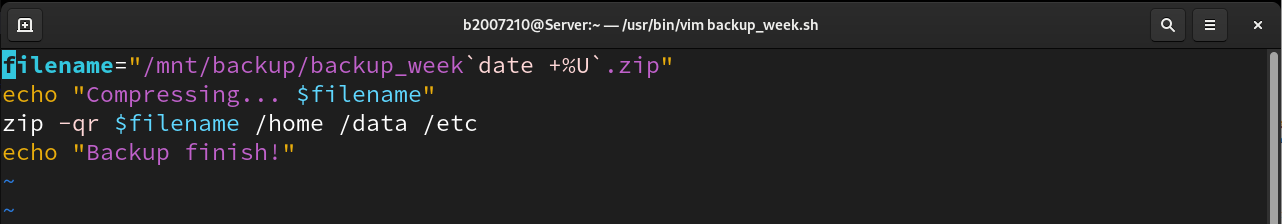
\includegraphics[width=\linewidth]{images/backup-week.png}
    \caption{Script backup mỗi tuần}
    \label{figure:backup-week}
\end{minipage}

\begin{lstlisting}[language=bash, caption={Script backup mỗi tuần}]
filename="/mnt/backup/backup_week$(date +%U).zip"
echo "Compressing... $filename"
zip -qr $filename /home /data /etc
echo "Backup finish!"
\end{lstlisting}

\begin{minipage}
    {\linewidth}
    \captionsetup{type=figure}
    \centering
    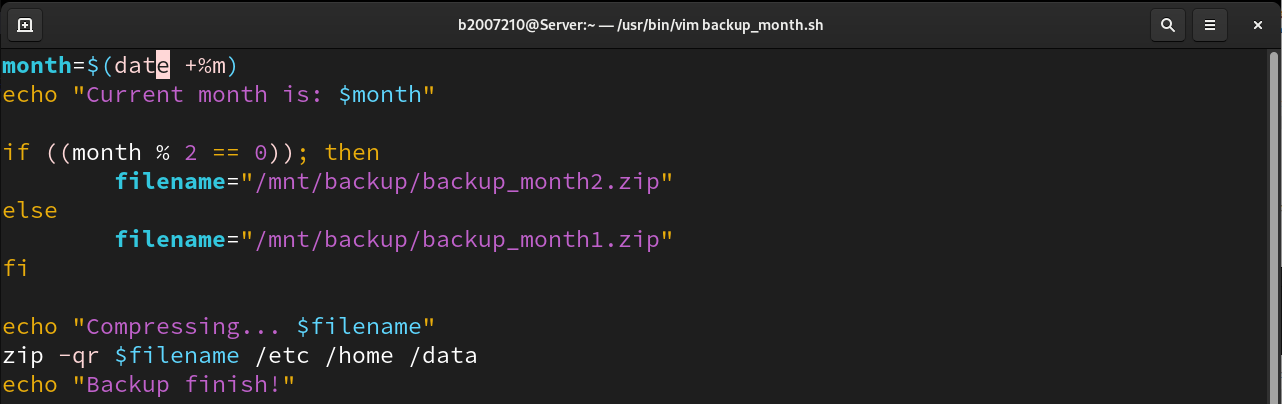
\includegraphics[width=\linewidth]{images/backup-month.png}
    \caption{Script backup mỗi tháng}
    \label{figure:backup-month}
\end{minipage}

\begin{lstlisting}[language=bash, caption={Script backup mỗi tháng}]
month=$(date +%m)
echo "Current month is: $month"

if ((month % 2 == 0))
then
    filename="/mnt/backup/backup_month2.zip"
else
    filename="/mnt/backup/backup_month1.zip"
fi

echo "Compressing... $filename"
zip -qr $filename /home /data /etc
echo "Backup finish!"
\end{lstlisting}

Ta sẽ lưu các script này vào các file \texttt{backup\_day.sh}, \texttt{backup\_week.sh}, \texttt{backup\_month.sh} trong thư mục \texttt{/mnt/backup}.

\subsubsection{Cấu hình cron}

Ta sẽ cấu hình cron để thực hiện script backup theo yêu cầu.

\begin{minipage}
    {\linewidth}
    \captionsetup{type=figure}
    \centering
    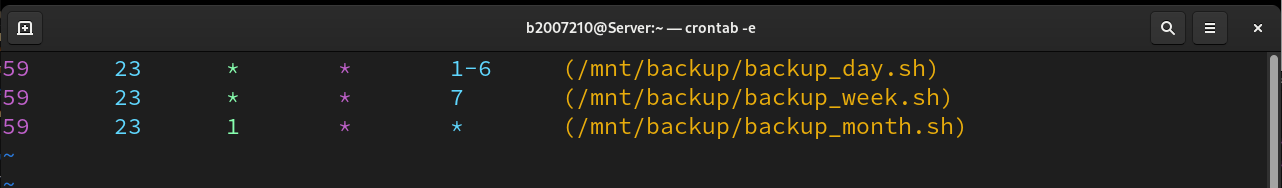
\includegraphics[width=\linewidth]{images/crontab.png}
    \caption{Cấu hình cron}
    \label{figure:crontab}
\end{minipage}

\begin{lstlisting}[language=bash, caption={Cấu hình cron}]
59  23  *   *   1-6 (/mnt/backup/backup_day.sh)
59  23  *   *   0   (/mnt/backup/backup_week.sh)
59  23  1   *   *   (/mnt/backup/backup_month.sh)
\end{lstlisting}

\end{document}